\documentclass[12pt,a4paper]{article}
\usepackage[a4paper, margin=0.8in, headheight=14pt]{geometry}
\usepackage{fontspec}
\usepackage{unicode-math}
\setmainfont{TeX Gyre Pagella}
\setmonofont[Scale=0.88]{TeX Gyre Cursor}
\setmathfont{Latin Modern Math}
\usepackage{xcolor}
\usepackage{colortbl}
\usepackage{titlesec}
\usepackage{enumitem}
\usepackage{tabularx}
\usepackage{booktabs}
\usepackage{array}
\usepackage{amsmath}
\usepackage{tikz}
\usetikzlibrary{shapes.geometric, arrows.meta, positioning, calc, fit, decorations.pathreplacing, decorations.pathmorphing}
\usepackage{tcolorbox}
\tcbuselibrary{skins, breakable}
\usepackage{hyperref}
\usepackage{fancyhdr}
\usepackage{graphicx}
\usepackage{microtype}
\hyphenpenalty=10000
\exhyphenpenalty=10000
\sloppy
\usepackage{caption}
\usepackage{setspace}
\usepackage{multirow}
\usepackage{tocloft}
\newcommand{\Q}[1]{\textbf{#1}\par\noindent\ignorespaces}
\definecolor{myred}{RGB}{196,30,58}
\definecolor{mydark}{RGB}{30,30,50}
\definecolor{mygreen}{RGB}{14,120,80}
\definecolor{myteal}{RGB}{0,130,140}
\definecolor{myamber}{RGB}{180,100,0}
\definecolor{mypurple}{RGB}{100,30,160}
\definecolor{mygray}{RGB}{246,247,249}
\definecolor{mgframe}{RGB}{180,185,200}
\definecolor{watermark}{RGB}{145,150,170}
\definecolor{hdrred}{RGB}{250,232,235}
\definecolor{hdrgreen}{RGB}{220,244,233}
\definecolor{hdrteal}{RGB}{220,242,244}
\definecolor{hdramber}{RGB}{253,242,215}
\definecolor{hdrpurple}{RGB}{238,228,255}
\definecolor{hdrgray}{RGB}{238,240,245}
\definecolor{rowalt}{RGB}{250,251,253}

\titleformat{\section}{\large\bfseries\color{myred}}{\thesection.}{0.5em}{}[\vspace{1pt}{\color{myred}\rule{\linewidth}{0.8pt}}]
\titleformat{\subsection}{\normalsize\bfseries\color{myteal}}{\thesubsection}{0.5em}{}
\titlespacing*{\section}{0pt}{18pt}{7pt}
\titlespacing*{\subsection}{0pt}{11pt}{4pt}
\setlength{\parindent}{0pt}
\setlength{\parskip}{4pt}
\renewcommand{\cfttoctitlefont}{\large\bfseries\color{myred}}
\renewcommand{\cftaftertoctitle}{\par\noindent{\color{myred}\rule{\linewidth}{0.8pt}}}
\setlength{\cftbeforetoctitleskip}{0pt}
\setlength{\cftaftertoctitleskip}{6pt}
\renewcommand{\cftsecfont}{\normalsize\bfseries\color{mydark}}
\renewcommand{\cftsecpagefont}{\normalsize\bfseries\color{mydark}}
\renewcommand{\cftsecleader}{\cftdotfill{\cftdotsep}}
\setlength{\cftbeforesecskip}{7pt}
\renewcommand{\cftsubsecfont}{\small\color{mydark}}
\renewcommand{\cftsubsecpagefont}{\small\color{mydark}}
\setlength{\cftbeforesubsecskip}{3pt}
\setlength{\cftsubsecindent}{1.4em}
\renewcommand{\cftpartfont}{\normalsize\bfseries\color{myteal}}
\renewcommand{\cftpartpagefont}{\normalsize\bfseries\color{myteal}}
\setlength{\cftbeforepartskip}{14pt}
\renewcommand{\arraystretch}{1.45}
\setlength{\tabcolsep}{6pt}
\arrayrulecolor{mydark}
\newcolumntype{B}[1]{>{\small\bfseries\raggedright\arraybackslash}m{#1}}
\newcolumntype{C}[1]{>{\centering\arraybackslash}m{#1}}
\newcolumntype{Y}{>{\small\raggedright\arraybackslash}X}
\renewcommand{\tabularxcolumn}[1]{m{#1}}
\newcommand{\currmodule}{Module 1}
\pagestyle{fancy}
\fancyhf{}
\fancyhead[L]{\small\color{myred}\textbf{PE-EC702A}\;\color{mydark}--- Adaptive Signal Processing}
\fancyhead[R]{\small\color{myteal}\textbf{\currmodule\ Notes}}
\fancyfoot[C]{\small\color{mydark}\thepage}
\fancyfoot[R]{\small\color{watermark}\textit{\copyright\ Biraj}}
\renewcommand{\headrulewidth}{0.5pt}
\renewcommand{\footrulewidth}{0.3pt}

\hypersetup{colorlinks=true, linkcolor=myteal, urlcolor=myteal,
  pdfauthor={Biraj Sarkar},
  pdftitle={PE-EC702A --- Combined Notes}}

\tcbset{
  tikzbox/.style={
    colback=mygray, colframe=mgframe, boxrule=0.6pt, arc=4pt,
    left=8pt, right=8pt, top=6pt, bottom=6pt,
    colbacktitle=mgframe, coltitle=mydark,
    fonttitle=\small\bfseries
  },
  defbox/.style={
    colback=hdrgreen, colframe=mygreen, boxrule=0.8pt, arc=4pt,
    left=9pt, right=9pt, top=6pt, bottom=6pt,
    colbacktitle=mygreen, coltitle=white,
    fonttitle=\small\bfseries
  },
  formulabox/.style={
    colback=hdrteal, colframe=myteal, boxrule=0.8pt, arc=4pt,
    left=9pt, right=9pt, top=7pt, bottom=7pt,
    colbacktitle=myteal, coltitle=white,
    fonttitle=\small\bfseries
  },
  examplebox/.style={
    colback=hdramber, colframe=myamber, boxrule=0.8pt, arc=4pt,
    left=9pt, right=9pt, top=6pt, bottom=6pt,
    colbacktitle=myamber, coltitle=white,
    fonttitle=\small\bfseries
  },
  masonbox/.style={
    colback=hdrpurple, colframe=mypurple, boxrule=0.8pt, arc=4pt,
    left=9pt, right=9pt, top=6pt, bottom=6pt,
    colbacktitle=mypurple, coltitle=white,
    fonttitle=\small\bfseries
  },
  exambox/.style={
    colback=hdrpurple, colframe=mypurple, boxrule=1pt, arc=5pt,
    left=10pt, right=10pt, top=8pt, bottom=8pt,
    colbacktitle=mypurple, coltitle=white,
    fonttitle=\bfseries,
    breakable, title after break={\textbf{Frequently Asked / Viva Questions (contd.)}}}
}
\tcbset{after={\color{black}}}

\tikzset{
  block/.style={rectangle, draw=myteal, fill=hdrteal,
    text width=2.4cm, align=center, minimum height=0.95cm,
    font=\small, rounded corners=3pt, line width=0.7pt},
  redblock/.style={rectangle, draw=myred, fill=hdrred,
    text width=2.4cm, align=center, minimum height=0.95cm,
    font=\small, rounded corners=3pt, line width=0.7pt},
  netnode/.style={rectangle, draw=myteal, fill=hdrteal,
    text width=1.5cm, align=center, minimum height=0.8cm,
    font=\small, rounded corners=3pt, line width=0.7pt},
  sumjunc/.style={circle, draw=myamber, fill=hdramber,
    minimum size=0.62cm, font=\small, line width=0.8pt},
  snode/.style={circle, draw=mypurple, fill=hdrpurple,
    minimum size=0.55cm, font=\footnotesize, line width=0.7pt},
  arrow/.style={-Stealth, thick, color=mydark},
  redarrow/.style={-Stealth, thick, color=myred},
  line/.style={thick, color=mydark}
}

\newcommand{\modulestart}[2]{%
  \clearpage
  \renewcommand{\currmodule}{Module #1}%
  \phantomsection
  \addcontentsline{toc}{part}{Module #1: #2}%
  \setcounter{section}{0}%
  \begin{center}
    \vspace*{1.0cm}
    {\Huge\bfseries\color{myred} Module #1}\\[10pt]
    {\Large\bfseries\color{mydark} #2}\\[10pt]
    {\color{myred}\rule{0.55\linewidth}{1.2pt}}
  \end{center}
  \vspace{14pt}
}
\begin{document}

\thispagestyle{empty}
\vspace*{1.0cm}
\begin{center}
  {\Huge\bfseries\color{myred} PE-EC702A}\\[10pt]
  {\LARGE\bfseries\color{mydark} Adaptive Signal Processing}\\[20pt]
  {\color{myred}\rule{0.7\linewidth}{1.5pt}}\\[18pt]
  {\Large\color{myteal}\textbf{Combined Module Notes}}\\[8pt]
  {\large\color{mydark} Modules 1 -- 5}\\[40pt]
  {\normalsize\color{mydark} Semester VII \quad$\bullet$\quad 3L:0T:0P \quad$\bullet$\quad 3 Credits}\\[12pt]
  {\normalsize\color{mydark} CGEC \;$|$\; B.Tech ECE (2023--27)}\\[6pt]
  {\normalsize\color{mydark}\textit{Biraj Sarkar}}
\end{center}
\vspace{1.0cm}
\begin{center}
  \begin{tcolorbox}[colback=mygray, colframe=mgframe, boxrule=0.5pt, arc=3pt, width=0.85\linewidth]
    \centering\small\color{mydark}
    \textbf{Disclaimer / Study Guide Notice:}\\
    These are condensed \textbf{Short Notes} focusing on core theory, key formulas, block/circuit diagrams, and standard viva Q\&As for university exam revision. Exhaustive numerical practice problems and derivation edge cases are not covered. This serves as a quick-revision reference guide for students.
  \end{tcolorbox}
\end{center}
\vfill
\begin{center}{\small\color{watermark}\textit{Exam-Ready Notes}}\end{center}
\clearpage

\hypersetup{linkcolor=mydark}
\tableofcontents
\hypersetup{linkcolor=myteal}
\clearpage

% -- Module 1 -----------------------------------------------------------------
\modulestart{1}{General Concept of Adaptive Filtering and Estimation}

\section{General Concept of Adaptive Filtering and Estimation}
% ===============================================================================

An adaptive filter is a self-designing, time-varying system that uses a recursive algorithm to adjust its parameters (coefficients) in order to minimize a predetermined cost function. Unlike fixed linear filters (e.g., standard FIR or IIR filters designed with static cutoff frequencies), adaptive filters automatically adjust to changes in the environment or statistics of the input signals.

\begin{tcolorbox}[defbox]
\textbf{Adaptive Filter:} A digital filter whose transfer function is automatically updated by an adaptive algorithm in response to an incoming error signal, which is computed as the difference between a desired response and the filter's actual output.
\end{tcolorbox}

\subsection{Basic Principles of Operation}
The operations of a typical adaptive filter are structured into two distinct stages:
\begin{enumerate}[label=\textbf{\arabic*.}, leftmargin=*, itemsep=3pt]
  \item \textbf{Filtering Process:} The filter processes an input signal $x(n)$ to produce an output signal $y(n)$. For an $M$-tap transversal (FIR) filter, this is represented by:
  \begin{equation}
    y(n) = \sum_{k=0}^{M-1} w_k(n) x(n-k) = \mathbf{w}^T(n) \mathbf{x}(n)
  \end{equation}
  where $\mathbf{w}(n) = [w_0(n), w_1(n), \dots, w_{M-1}(n)]^T$ is the weight vector, and $\mathbf{x}(n) = [x(n), x(n-1), \dots, x(n-M+1)]^T$ is the input vector.
  \item \textbf{Adaptive Process (Feedback):} An error signal $e(n)$ is generated by comparing the filter output $y(n)$ with a desired response $d(n)$:
  \begin{equation}
    e(n) = d(n) - y(n)
  \end{equation}
  The adaptive algorithm (e.g., LMS or RLS) uses this error $e(n)$ to update the filter coefficients for the next time index:
  \begin{equation}
    \mathbf{w}(n+1) = \mathbf{w}(n) + \Delta \mathbf{w}(n)
  \end{equation}
\end{enumerate}

\subsection{Adaptive Filter Block Diagram}
The schematic block diagram below represents the closed-loop feedback structure of an adaptive filter:

\begin{tcolorbox}[tikzbox, title={Adaptive Filter Closed-Loop Block Diagram}]
\centering
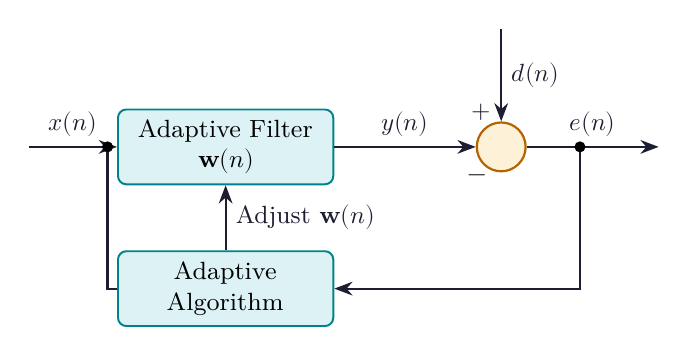
\begin{tikzpicture}[node distance=0.8cm and 1.2cm, every node/.style={font=\small}]
  \coordinate (input) at (-1.5, 0);
  \node[block, text width=2.5cm] (filter) at (1.0, 0) {Adaptive Filter\\$\mathbf{w}(n)$};
  \node[sumjunc] (sum) at (4.5, 0) {};
  \node[block, text width=2.5cm] (algo) at (1.0, -1.8) {Adaptive Algorithm};
  \coordinate (desired) at (4.5, 1.5);
  \coordinate (output) at (6.5, 0);
  
  \draw[arrow] (input) -- node[midway, above] {$x(n)$} (filter);
  \draw[line] (-0.5, 0) |- (algo.west);
  \fill (-0.5, 0) circle (2pt);
  
  \draw[arrow] (filter) -- node[midway, above] {$y(n)$} (sum);
  \draw[arrow] (desired) -- node[midway, right] {$d(n)$} node[pos=0.9, left] {$+$} (sum);
  \draw[arrow] (sum) -- node[midway, above] {$e(n)$} (output);
  \draw[arrow] (5.5, 0) |- (algo.east);
  \fill (5.5, 0) circle (2pt);
  
  \draw[arrow] (algo.north) -- node[midway, right] {Adjust $\mathbf{w}(n)$} (filter.south);
  \node at (4.2, -0.4) {$-$};
\end{tikzpicture}
\end{tcolorbox}

% ===============================================================================
\section{Applications and Motivation}
% ===============================================================================

The primary motivation for adaptive filtering is the inability of classical filter designs to operate in environments where the signal characteristics are either unknown or time-varying. Typical applications are categorized into four basic classes depending on the choice of input $x(n)$ and desired response $d(n)$:

\subsection{The Four Classes of Adaptive Filter Applications}

\begin{enumerate}[label=\textbf{\arabic*.}, leftmargin=*, itemsep=4pt]
  \item \textbf{System Identification:} The adaptive filter models the transfer function of an unknown system.
    \begin{itemize}[label=$\bullet$, leftmargin=*]
      \item \textit{Setup:} Input $x(n)$ is fed to both the unknown system and the adaptive filter. The system output is the desired response $d(n)$.
      \item \textit{Application:} Echo cancellation in long-distance telephony, channel characterization.
    \end{itemize}
  \item \textbf{Inverse Modeling (Equalization):} The filter is placed in cascade with an unknown channel to compensate for channel distortion.
    \begin{itemize}[label=$\bullet$, leftmargin=*]
      \item \textit{Setup:} A known training signal is sent. The distorted channel output is input $x(n)$, and the original training signal is the desired response $d(n)$.
      \item \textit{Application:} High-speed digital communication channel equalization.
    \end{itemize}
  \item \textbf{Noise Cancellation (Interference Cancellation):} The filter estimates and subtracts noise from a corrupted signal.
    \begin{itemize}[label=$\bullet$, leftmargin=*]
      \item \textit{Setup:} Input $x(n)$ is a reference noise source. The desired response $d(n)$ is the signal corrupted by noise.
      \item \textit{Application:} Active noise control, cancellation of maternal ECG in fetal monitoring.
    \end{itemize}
  \item \textbf{Linear Prediction:} The filter predicts future values of a random process.
    \begin{itemize}[label=$\bullet$, leftmargin=*]
      \item \textit{Setup:} Input $x(n)$ is a delayed version of the signal, and the desired response $d(n)$ is the current signal value.
      \item \textit{Application:} Linear Predictive Coding (LPC) in speech compression, ADPCM encoders.
    \end{itemize}
\end{enumerate}

\par\noindent
\begin{tabularx}{\linewidth}{|B{3.2cm}|Y|Y|Y|}
\hline
\rowcolor{hdrteal}
\textbf{Application Class} & \textbf{Input Signal $x(n)$} & \textbf{Desired Signal $d(n)$} & \textbf{Objective} \\
\hline
\textbf{System ID} & Reference excitation & Unknown system output & Find model $\mathbf{w}(n) \approx \text{system}$ \\
\hline
\rowcolor{rowalt}
\textbf{Inverse Model} & Distorted signal & Original source signal & Recover original source \\
\hline
\textbf{Noise Cancellation} & Noise reference source & Corrupted signal & Extract clean signal $e(n)$ \\
\hline
\rowcolor{rowalt}
\textbf{Prediction} & Delayed signal $s(n-\Delta)$ & Current signal $s(n)$ & Predict future signal values \\
\hline
\end{tabularx}

% ===============================================================================
\section{Review of Probability, Random Variables and Stationary Processes}
% ===============================================================================

Adaptive filter design relies heavily on statistical signal processing. This section reviews the prerequisite concepts of random signals.

\subsection{Random Variables and Probability Density Functions}
A random variable $X$ is a mapping from sample space to real numbers. It is described by its Probability Density Function (PDF) $f_X(x)$.
\begin{itemize}[leftmargin=*, itemsep=2pt]
  \item \textbf{Expectation (Mean):} The statistical average of $X$:
  \begin{equation}
    \mu_X = \mathbb{E}[X] = \int_{-\infty}^{\infty} x f_X(x) \, dx
  \end{equation}
  \item \textbf{Variance:} The measure of signal spread/power:
  \begin{equation}
    \sigma_X^2 = \mathbb{E}[(X - \mu_X)^2] = \mathbb{E}[X^2] - \mu_X^2
  \end{equation}
\end{itemize}

\subsection{Stationary and Ergodicity}
A random process $X(n)$ is a collection of random variables indexed by time.
\begin{itemize}[leftmargin=*, itemsep=3pt]
  \item \textbf{Strict-Sense Stationarity (SSS):} A process is SSS if its joint probability distributions are invariant to any shift in the time origin.
  \item \textbf{Wide-Sense Stationarity (WSS):} A process is WSS if:
    \begin{enumerate}[label=\textbf{\alph*.}, leftmargin=*, itemsep=1pt]
      \item Its mean is constant over time: $\mathbb{E}[X(n)] = \mu$
      \item Its autocorrelation depends only on the time difference (lag) $k$:
      \begin{equation}
        R_x(k) = \mathbb{E}[X(n) X^*(n-k)]
      \end{equation}
    \end{enumerate}
  \item \textbf{Ergodicity:} A WSS process is ergodic if its time averages equal its ensemble averages. This allows computing statistical metrics from a single, long time realization.
\end{itemize}

% ===============================================================================
\section{Correlation Structures and Correlation Matrices}
% ===============================================================================

Let $\mathbf{x}(n) = [x(n), x(n-1), \dots, x(n-M+1)]^T$ be an $M \times 1$ tap-input vector of a WSS process. The statistical relationship among its elements is captured by the autocorrelation matrix $\mathbf{R}$.

\subsection{The Autocorrelation Matrix}
The autocorrelation matrix $\mathbf{R}$ is defined as:
\begin{equation}
  \mathbf{R} = \mathbb{E}[\mathbf{x}(n) \mathbf{x}^H(n)]
\end{equation}
where $^H$ denotes the Hermitian transpose (conjugate transpose). In expanded form:
\begin{equation}
  \mathbf{R} = \begin{bmatrix}
    R_x(0) & R_x(1) & \dots & R_x(M-1) \\
    R_x(-1) & R_x(0) & \dots & R_x(M-2) \\
    \vdots & \vdots & \ddots & \vdots \\
    R_x(-M+1) & R_x(-M+2) & \dots & R_x(0)
  \end{bmatrix}
\end{equation}
Since the process is WSS, $R_x(-k) = R_x^*(k)$.

\subsection{Properties of the Correlation Matrix}
The matrix $\mathbf{R}$ possesses several fundamental properties that dictate the behavior of adaptive filters:
\begin{enumerate}[label=\textbf{\arabic*.}, leftmargin=*, itemsep=4pt]
  \item \textbf{Hermitian Symmetry:} $\mathbf{R}$ is Hermitian, i.e., $\mathbf{R}^H = \mathbf{R}$.
  \item \textbf{Toeplitz Structure:} All elements along any main diagonal are identical. This symmetry reduces computational cost for matrix inversion algorithms.
  \item \textbf{Positive Semi-Definiteness:} For any non-zero complex vector $\mathbf{a}$:
  \begin{equation}
    \mathbf{a}^H \mathbf{R} \mathbf{a} = \mathbf{a}^H \mathbb{E}[\mathbf{x}(n)\mathbf{x}^H(n)]\mathbf{a} = \mathbb{E}[|\mathbf{a}^H\mathbf{x}(n)|^2] \ge 0
  \end{equation}
  If no component of the input signal is perfectly predictable, $\mathbf{R}$ is positive definite ($\mathbf{a}^H \mathbf{R} \mathbf{a} > 0$), meaning all its eigenvalues are strictly positive ($\lambda_i > 0$), ensuring $\mathbf{R}$ is invertible.
  \item \textbf{Eigenvalue Bounds:} The eigenvalues of $\mathbf{R}$ are bounded by the minimum and maximum values of the Power Spectral Density (PSD) of the input process:
  \begin{equation}
    S_{\text{min}} \le \lambda_i \le S_{\text{max}}
  \end{equation}
\end{enumerate}

\begin{tcolorbox}[examplebox, title={Example: Correlation Matrix of a Sinusoid with Noise}]
Consider an input signal $x(n) = A \cos(\omega_0 n + \theta) + v(n)$, where $\theta$ is uniformly distributed in $[-\pi, \pi]$ and $v(n)$ is zero-mean white noise with variance $\sigma_v^2$ uncorrelated with the sinusoid. Compute the autocorrelation matrix for $M = 2$.

\textbf{Solution:}
The autocorrelation function of the sinusoid is $R_s(k) = \frac{A^2}{2}\cos(\omega_0 k)$.
The autocorrelation function of the white noise is $R_v(k) = \sigma_v^2 \delta(k)$.
Since they are uncorrelated, the total autocorrelation is:
\[
  R_x(k) = R_s(k) + R_v(k) = \frac{A^2}{2}\cos(\omega_0 k) + \sigma_v^2 \delta(k)
\]
For $k=0$ and $k=1$:
\[
  R_x(0) = \frac{A^2}{2} + \sigma_v^2
\]
\[
  R_x(1) = \frac{A^2}{2}\cos(\omega_0)
\]
Thus, the $2 \times 2$ correlation matrix is:
\[
  \mathbf{R} = \begin{bmatrix}
    \frac{A^2}{2} + \sigma_v^2 & \frac{A^2}{2}\cos(\omega_0) \\
    \frac{A^2}{2}\cos(\omega_0) & \frac{A^2}{2} + \sigma_v^2
  \end{bmatrix}
\]
\end{tcolorbox}

% ===============================================================================
% MANDATORY QUICK REVISION PAGE
% ===============================================================================
\newpage
\begin{center}
  {\large\bfseries\color{myred} Quick Revision --- Module I}\\[3pt]
  {\small\color{mydark} Adaptive Filtering Concepts \& Random Processes $|$ PE-EC702A}
\end{center}
\noindent{\color{myred}\rule{\linewidth}{1.2pt}}
\vspace{4pt}

\begin{tcolorbox}[formulabox, title={\textbf{Key Formulas at a Glance}}]
\renewcommand{\arraystretch}{1.3}
\begin{tabularx}{\linewidth}{B{4.5cm} X}
Filter Output (FIR) & $y(n) = \mathbf{w}^T(n)\mathbf{x}(n) = \sum_{k=0}^{M-1} w_k(n) x(n-k)$ \\[6pt]
Error Signal & $e(n) = d(n) - y(n)$ \\[6pt]
Autocorrelation Function & $R_x(k) = \mathbb{E}[x(n) x^*(n-k)]$ \\[6pt]
Correlation Matrix & $\mathbf{R} = \mathbb{E}[\mathbf{x}(n) \mathbf{x}^H(n)]$ \\[6pt]
Cross-Correlation Vector & $\mathbf{p} = \mathbb{E}[\mathbf{x}(n) d^*(n)]$
\end{tabularx}
\end{tcolorbox}

\begin{tcolorbox}[defbox, title={\textbf{One-Line Definitions}}]
\begin{itemize}[leftmargin=*, itemsep=2.5pt, topsep=0pt]
  \item \textbf{Adaptive Filter:} A digital filter that dynamically self-adjusts its coefficients to minimize a cost function.
  \item \textbf{Desired Response:} The target reference signal that the adaptive filter output attempts to replicate.
  \item \textbf{Wide-Sense Stationarity:} A process with constant mean and an autocorrelation depending only on lag.
  \item \textbf{Ergodicity:} A property where time-average statistics are identical to ensemble-average statistics.
  \item \textbf{Toeplitz Matrix:} A matrix where elements on each diagonal are constant, characteristic of WSS correlation matrices.
  \item \textbf{Hermitian Matrix:} A complex matrix equal to its own conjugate transpose, $\mathbf{R}^H = \mathbf{R}$.
\end{itemize}
\end{tcolorbox}

\begin{tcolorbox}[exambox, title={\textbf{Frequently Asked / Viva Questions}}]
\begin{enumerate}[topsep=0pt, label=\textbf{Q\arabic*.}, itemsep=5pt]
  \item \Q{What is the primary difference between a fixed filter and an adaptive filter?}
    Fixed filters have static coefficients designed based on prior knowledge of signal spectra, whereas adaptive filters continuously update their coefficients in real-time based on statistical changes in the input signals.
  \item \Q{Explain the role of the desired response $d(n)$ in an adaptive system.}
    The desired response acts as a target reference signal. The difference between $d(n)$ and the filter output $y(n)$ produces the error $e(n)$, which guides the optimization algorithm.
  \item \Q{Identify the four main application classes of adaptive filters.}
    System Identification, Inverse Modeling (Equalization), Noise Cancellation, and Linear Prediction.
  \item \Q{Why does the autocorrelation matrix $\mathbf{R}$ of a WSS process possess Toeplitz structure?}
    Because for a WSS process, the autocorrelation between $x(i)$ and $x(j)$ depends strictly on the lag $|i - j|$, causing elements along any diagonal to be identical.
  \item \Q{State the significance of the positive definite property of a correlation matrix.}
    Positive definiteness implies that all eigenvalues of $\mathbf{R}$ are strictly positive ($\lambda_i > 0$), which guarantees that the matrix is non-singular and hence invertible.
  \item \Q{What is ensemble average vs time average?}
    Ensemble average is the average across all possible realizations of a random variable at a specific time, while time average is computed along a single realization over infinite time.
  \item \Q{Define a Hermitian matrix in the context of adaptive filtering.}
    A matrix $\mathbf{R}$ is Hermitian if $\mathbf{R}^H = \mathbf{R}$ (where $^H$ denotes the conjugate transpose). The autocorrelation matrix of any complex random process is always Hermitian.
  \item \Q{What is the physical interpretation of $R_x(0)$?}
    $R_x(0) = \mathbb{E}[|x(n)|^2]$, which represents the average total power of the input signal $x(n)$.
  \item \Q{What happens to the eigenvalues of $\mathbf{R}$ if the input is white noise?}
    All eigenvalues of the correlation matrix of white noise are identical and equal to the noise variance ($\lambda_i = \sigma^2$).
  \item \Q{What is the cross-correlation vector $\mathbf{p}$?}
    It is the statistical correlation vector between the input signal vector $\mathbf{x}(n)$ and the desired response $d(n)$, defined as $\mathbf{p} = \mathbb{E}[\mathbf{x}(n) d^*(n)]$.
\end{enumerate}
\end{tcolorbox}

\begin{tcolorbox}[tikzbox, title={Comparison of Adaptive Filter Application Classes}]
\renewcommand{\arraystretch}{1.4}
\par\noindent
\begin{tabularx}{\linewidth}{|B{2.8cm}|Y|Y|Y|}
\hline
\rowcolor{hdrgray}
\textbf{Parameter} & \textbf{System ID} & \textbf{Noise Cancellation} & \textbf{Equalization} \\
\hline
\textbf{Filter Input $x(n)$} & Excitation signal & Reference noise source & Distorted channel output \\
\hline
\textbf{Desired Input $d(n)$} & Output of unknown system & Corrupted signal & Known training signal \\
\hline
\textbf{Desired Output} & Model of system parameters & Cleaned signal $e(n)$ & Reconstructed original data \\
\hline
\textbf{Key Application} & Echo cancellation in telephony & Active noise control, EEG & Wireless communications \\
\hline
\end{tabularx}
\end{tcolorbox}


% -- Module 2 -----------------------------------------------------------------
\modulestart{2}{Optimal FIR (Wiener) Filter}

\section{Optimal FIR (Wiener) Filter}
% ===============================================================================

The Wiener filter is the optimal linear filter in the Mean-Square Error (MSE) sense. It assumes the signals are wide-sense stationary with known second-order statistics (autocorrelation and cross-correlation).

\subsection{Derivation of the Wiener-Hopf Equations}
Let the input vector be $\mathbf{x}(n) = [x(n), x(n-1), \dots, x(n-M+1)]^T$ and the weight vector be $\mathbf{w} = [w_0, w_1, \dots, w_{M-1}]^T$. The filter output is $y(n) = \mathbf{w}^H \mathbf{x}(n)$. The error signal is $e(n) = d(n) - y(n) = d(n) - \mathbf{w}^H \mathbf{x}(n)$.
The cost function to minimize is the Mean-Square Error $J(\mathbf{w}) = \mathbb{E}[|e(n)|^2]$:
\begin{equation}
  J(\mathbf{w}) = \mathbb{E}\left[(d(n) - \mathbf{w}^H \mathbf{x}(n))(d^*(n) - \mathbf{x}^H(n) \mathbf{w})\right]
\end{equation}
Expanding the expectation:
\begin{align}
  J(\mathbf{w}) &= \mathbb{E}[|d(n)|^2] - \mathbf{w}^H \mathbb{E}[\mathbf{x}(n) d^*(n)] - \mathbb{E}[d(n) \mathbf{x}^H(n)] \mathbf{w} + \mathbf{w}^H \mathbb{E}[\mathbf{x}(n) \mathbf{x}^H(n)] \mathbf{w} \nonumber \\
  &= \sigma_d^2 - \mathbf{w}^H \mathbf{p} - \mathbf{p}^H \mathbf{w} + \mathbf{w}^H \mathbf{R} \mathbf{w}
\end{align}
where $\sigma_d^2 = \mathbb{E}[|d(n)|^2]$, $\mathbf{p} = \mathbb{E}[\mathbf{x}(n) d^*(n)]$, and $\mathbf{R} = \mathbb{E}[\mathbf{x}(n) \mathbf{x}^H(n)]$.
To find the optimal weight vector $\mathbf{w}_o$, we differentiate $J(\mathbf{w})$ with respect to the complex conjugate of the weight vector $\mathbf{w}^*$ (or compute the gradient) and set it to zero:
\begin{equation}
  \nabla_{\mathbf{w}^*} J(\mathbf{w}) = -\mathbf{p} + \mathbf{R} \mathbf{w} = \mathbf{0}
\end{equation}
This yields the \textbf{Wiener-Hopf Equations}:
\begin{equation}
  \mathbf{R} \mathbf{w}_o = \mathbf{p} \implies \mathbf{w}_o = \mathbf{R}^{-1} \mathbf{p}
\end{equation}

\subsection{Minimum Mean-Square Error (\texorpdfstring{$J_{\text{min}}$}{Jmin})}
Substituting the optimal weight $\mathbf{w}_o$ back into the cost function $J(\mathbf{w})$ gives the minimum mean-square error:
\begin{equation}
  J_{\text{min}} = \sigma_d^2 - \mathbf{w}_o^H \mathbf{p} = \sigma_d^2 - \mathbf{p}^H \mathbf{R}^{-1} \mathbf{p}
\end{equation}

% ===============================================================================
\section{Method of Steepest Descent}
% ===============================================================================

When the statistics $\mathbf{R}$ and $\mathbf{p}$ are known, but inverting $\mathbf{R}$ is computationally expensive, we use the iterative Method of Steepest Descent. The weight vector is updated in the direction opposite to the gradient of the performance surface $J(\mathbf{w})$:

\subsection{Weight Update Equation}
\begin{equation}
  \mathbf{w}(n+1) = \mathbf{w}(n) - \frac{1}{2} \mu \nabla J(\mathbf{w}(n))
\end{equation}
where $\mu$ is the step-size parameter. Since $\nabla J(\mathbf{w}) = -2\mathbf{p} + 2\mathbf{R}\mathbf{w}(n)$, we have:
\begin{equation}
  \mathbf{w}(n+1) = \mathbf{w}(n) + \mu (\mathbf{p} - \mathbf{R} \mathbf{w}(n))
\end{equation}

\subsection{Convergence Analysis and Stability}
Let the weight error vector be defined as $\mathbf{c}(n) = \mathbf{w}(n) - \mathbf{w}_o$. Subtracting $\mathbf{w}_o$ from both sides of the update equation:
\begin{equation}
  \mathbf{c}(n+1) = (\mathbf{I} - \mu \mathbf{R})\mathbf{c}(n)
\end{equation}
Applying the spectral decomposition $\mathbf{R} = \mathbf{Q} \mathbf{\Lambda} \mathbf{Q}^H$ and defining the rotated error vector $\mathbf{v}(n) = \mathbf{Q}^H \mathbf{c}(n)$, we get:
\begin{equation}
  \mathbf{v}(n+1) = (\mathbf{I} - \mu \mathbf{\Lambda})\mathbf{v}(n)
\end{equation}
For stability, each decoupled mode $v_i(n+1) = (1 - \mu \lambda_i)v_i(n)$ must decay to zero, which requires $|1 - \mu \lambda_i| < 1$ for all $i$:
\begin{equation}
  0 < \mu < \frac{2}{\lambda_{\text{max}}}
\end{equation}
where $\lambda_{\text{max}}$ is the largest eigenvalue of the correlation matrix $\mathbf{R}$.

\begin{tcolorbox}[tikzbox, title={Contour Lines of MSE Surface and Convergence Trajectory}]
\centering
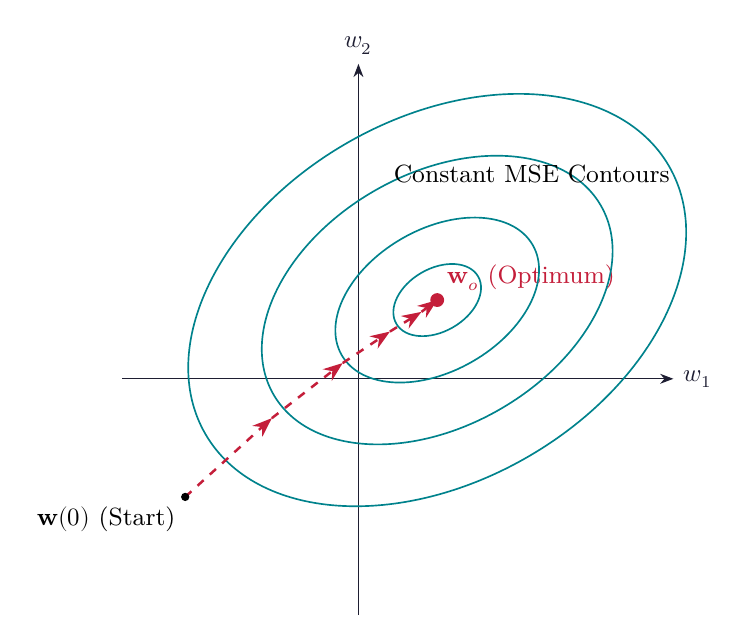
\begin{tikzpicture}[every node/.style={font=\small}]
  % Axes
  \draw[-Stealth, thin, color=mydark] (-3,0) -- (4,0) node[right] {$w_1$};
  \draw[-Stealth, thin, color=mydark] (0,-3) -- (0,4) node[above] {$w_2$};
  
  % Optimal Point
  \fill[color=myred] (1,1) circle (2.5pt) node[above right] {$\mathbf{w}_o$ (Optimum)};
  
  % Elliptical Contours
  \draw[color=myteal, semithick] (1,1) circle [x radius=0.6cm, y radius=0.4cm, rotate=30];
  \draw[color=myteal, semithick] (1,1) circle [x radius=1.4cm, y radius=0.9cm, rotate=30];
  \draw[color=myteal, semithick] (1,1) circle [x radius=2.4cm, y radius=1.6cm, rotate=30];
  \draw[color=myteal, semithick] (1,1) circle [x radius=3.4cm, y radius=2.3cm, rotate=30];
  
  % Trajectory path
  \draw[redarrow, dashed, line width=0.9pt] (-2.2,-1.5) -- (-1.1,-0.5);
  \draw[redarrow, dashed, line width=0.9pt] (-1.1,-0.5) -- (-0.2, 0.2);
  \draw[redarrow, dashed, line width=0.9pt] (-0.2, 0.2) -- (0.4, 0.6);
  \draw[redarrow, dashed, line width=0.9pt] (0.4, 0.6) -- (0.8, 0.85);
  \draw[redarrow, dashed, line width=0.9pt] (0.8, 0.85) -- (1.0, 1.0);
  
  \fill (-2.2,-1.5) circle (1.5pt) node[below left] {$\mathbf{w}(0)$ (Start)};
  \node at (2.2, 2.6) {Constant MSE Contours};
\end{tikzpicture}
\end{tcolorbox}

% ===============================================================================
\section{The Least Mean Squares (LMS) Algorithm}
% ===============================================================================

The Least Mean Squares (LMS) algorithm is a stochastic gradient descent algorithm. It avoids the need to know or estimate the ensemble statistics $\mathbf{R}$ and $\mathbf{p}$ by using instantaneous approximations:
\begin{equation}
  \hat{\mathbf{R}}(n) = \mathbf{x}(n) \mathbf{x}^H(n), \quad \hat{\mathbf{p}}(n) = \mathbf{x}(n) d^*(n)
\end{equation}

\subsection{LMS Algorithms Formulations}
The instantaneous cost function is chosen as $\hat{J}(n) = |e(n)|^2$. The update equations are:
\begin{tcolorbox}[defbox, title={LMS Update Equations}]
\textbf{Real-Valued LMS Algorithm:}
\begin{align}
  e(n) &= d(n) - \mathbf{w}^T(n) \mathbf{x}(n) \\
  \mathbf{w}(n+1) &= \mathbf{w}(n) + \mu e(n) \mathbf{x}(n)
\end{align}
\textbf{Complex-Valued LMS Algorithm:}
\begin{align}
  e(n) &= d(n) - \mathbf{w}^H(n) \mathbf{x}(n) \\
  \mathbf{w}(n+1) &= \mathbf{w}(n) + \mu \mathbf{x}(n) e^*(n)
\end{align}
\end{tcolorbox}

\subsection{LMS Convergence Analysis}
Under the \textbf{independence assumption} (the input vectors $\mathbf{x}(n)$ are statistically independent over time):
\begin{itemize}[leftmargin=*, itemsep=3pt]
  \item \textbf{Convergence in the Mean:} The ensemble average of the weights converges to the Wiener solution, $\mathbb{E}[\mathbf{w}(n)] \to \mathbf{w}_o$, if:
  \begin{equation}
    0 < \mu < \frac{2}{\lambda_{\text{max}}}
  \end{equation}
  A conservative practical limit based on total signal power is:
  \begin{equation}
    0 < \mu < \frac{2}{\text{Tr}(\mathbf{R})} = \frac{2}{M \cdot R_x(0)}
  \end{equation}
  \item \textbf{Convergence in the Mean-Square:} For the second-order statistics of the weights to remain stable, the step-size must satisfy:
  \begin{equation}
    0 < \mu < \frac{2}{\sum_{i=1}^M \lambda_i} = \frac{2}{\text{Tr}(\mathbf{R})}
  \end{equation}
\end{itemize}

\subsection{Excess MSE and Misadjustment}
Due to gradient estimation noise, the LMS algorithm does not settle exactly at $J_{\text{min}}$. It fluctuates about the optimum, introducing an \textbf{Excess Mean-Square Error} $J_{\text{ex}}$:
\begin{equation}
  J_{\text{ex}} = \lim_{n\to\infty} \mathbb{E}[|e(n)|^2] - J_{\text{min}}
\end{equation}
For a small step-size $\mu$, the excess MSE is given by:
\begin{equation}
  J_{\text{ex}} \approx \frac{\mu J_{\text{min}} \text{Tr}(\mathbf{R})}{2 - \mu \text{Tr}(\mathbf{R})}
\end{equation}
The \textbf{Misadjustment} $M$ is a dimensionless measure of how close the LMS filter is to the optimal Wiener filter:
\begin{equation}
  M = \frac{J_{\text{ex}}}{J_{\text{min}}} \approx \frac{\mu}{2} \text{Tr}(\mathbf{R}) = \frac{\mu}{2} \sum_{i=1}^M \lambda_i
\end{equation}

\begin{tcolorbox}[examplebox, title={Example: Wiener Filter Coefficient Design}]
A single-tap LMS filter has input signal $x(n)$ with variance $R_x(0) = 2$. The desired signal has variance $\sigma_d^2 = 5$, and the cross-correlation is $p = 1.6$. 
\begin{enumerate}[label=\textbf{\arabic*.}, leftmargin=*, itemsep=2pt]
  \item Determine the optimal weight $w_o$.
  \item Compute the minimum MSE $J_{\text{min}}$.
  \item Determine the maximum step-size $\mu$ for convergence in the mean.
  \item Calculate the misadjustment $M$ for $\mu = 0.05$.
\end{enumerate}

\textbf{Solution:}
\begin{enumerate}[label=\textbf{\arabic*.}, leftmargin=*, itemsep=4pt]
  \item Using the Wiener-Hopf equation:
    \[
      w_o = R^{-1}p = \frac{p}{R_x(0)} = \frac{1.6}{2} = 0.8
    \]
  \item The minimum MSE $J_{\text{min}}$ is:
    \[
      J_{\text{min}} = \sigma_d^2 - w_o p = 5 - (0.8 \times 1.6) = 5 - 1.28 = 3.72
    \]
  \item For a single-tap filter ($M=1$), $\lambda_{\text{max}} = R_x(0) = 2$. The step-size range is:
    \[
      0 < \mu < \frac{2}{\lambda_{\text{max}}} \implies 0 < \mu < 1
    \]
  \item The misadjustment $M$ for $\mu = 0.05$:
    \[
      M \approx \frac{\mu}{2} \text{Tr}(\mathbf{R}) = \frac{0.05}{2} \times 2 = 0.05 \text{ (or 5\%)}
    \]
\end{enumerate}
\end{tcolorbox}

% ===============================================================================
% MANDATORY QUICK REVISION PAGE
% ===============================================================================
\newpage
\begin{center}
  {\large\bfseries\color{myred} Quick Revision --- Module II}\\[3pt]
  {\small\color{mydark} Wiener Filters, Steepest Descent \& LMS $|$ PE-EC702A}
\end{center}
\noindent{\color{myred}\rule{\linewidth}{1.2pt}}
\vspace{4pt}

\begin{tcolorbox}[formulabox, title={\textbf{Key Formulas at a Glance}}]
\renewcommand{\arraystretch}{1.3}
\begin{tabularx}{\linewidth}{B{4.5cm} X}
Wiener-Hopf Equation & $\mathbf{R} \mathbf{w}_o = \mathbf{p} \implies \mathbf{w}_o = \mathbf{R}^{-1} \mathbf{p}$ \\[6pt]
Minimum MSE & $J_{\text{min}} = \sigma_d^2 - \mathbf{p}^H \mathbf{w}_o$ \\[6pt]
Steepest Descent Update & $\mathbf{w}(n+1) = \mathbf{w}(n) + \mu (\mathbf{p} - \mathbf{R}\mathbf{w}(n))$ \\[6pt]
LMS Update (Complex) & $\mathbf{w}(n+1) = \mathbf{w}(n) + \mu \mathbf{x}(n) e^*(n)$ \\[6pt]
Step-Size Bounds & $0 < \mu < \frac{2}{\lambda_{\text{max}}}$ \quad (Ensemble) or $0 < \mu < \frac{2}{\text{Tr}(\mathbf{R})}$ \quad (LMS) \\[6pt]
Misadjustment & $M = \frac{J_{\text{ex}}}{J_{\text{min}}} \approx \frac{\mu}{2} \text{Tr}(\mathbf{R})$
\end{tabularx}
\end{tcolorbox}

\begin{tcolorbox}[defbox, title={\textbf{One-Line Definitions}}]
\begin{itemize}[leftmargin=*, itemsep=2.5pt, topsep=0pt]
  \item \textbf{Wiener Filter:} The optimal linear time-invariant filter that minimizes mean-square error.
  \item \textbf{Steepest Descent:} An iterative optimization method that moves weights along the direction of maximum negative gradient.
  \item \textbf{LMS Algorithm:} A low-complexity adaptive algorithm using instantaneous signal values to approximate gradients.
  \item \textbf{Misadjustment:} A measure of the average excess MSE relative to the minimum MSE, representing algorithm noise.
  \item \textbf{Eigenvalue Spread:} The ratio $\lambda_{\text{max}}/\lambda_{\text{min}}$, indicating the convergence rate limit of gradient algorithms.
  \item \textbf{Independence Assumption:} An analytical simplification stating that successive tap-input vectors are statistically independent.
\end{itemize}
\end{tcolorbox}

\begin{tcolorbox}[exambox, title={\textbf{Frequently Asked / Viva Questions}}]
\begin{enumerate}[topsep=0pt, label=\textbf{Q\arabic*.}, itemsep=5pt]
  \item \Q{Derive the Wiener-Hopf equations for a real FIR filter.}
    See Section 1.1: We expand $J(\mathbf{w}) = \mathbb{E}[(d(n) - \mathbf{w}^T\mathbf{x}(n))^2] = \sigma_d^2 - 2\mathbf{w}^T\mathbf{p} + \mathbf{w}^T\mathbf{R}\mathbf{w}$. Differentiating w.r.t. $\mathbf{w}$ and setting to $\mathbf{0}$ yields $\mathbf{R}\mathbf{w}_o = \mathbf{p}$.
  \item \Q{What is the convergence criterion for the method of steepest descent?}
    The step-size parameter must satisfy $0 < \mu < 2/\lambda_{\text{max}}$, where $\lambda_{\text{max}}$ is the maximum eigenvalue of the autocorrelation matrix $\mathbf{R}$.
  \item \Q{Why is LMS referred to as a "stochastic" gradient algorithm?}
    Because it replaces the true gradient (which requires expectations of signals) with a noisy instantaneous gradient estimate computed directly from the current samples.
  \item \Q{Write down the complex LMS weight update equation and explain each term.}
    $\mathbf{w}(n+1) = \mathbf{w}(n) + \mu \mathbf{x}(n)e^*(n)$, where $\mathbf{w}(n)$ is the weight vector, $\mu$ is the step-size, $\mathbf{x}(n)$ is the input vector, and $e^*(n)$ is the complex conjugate of the error.
  \item \Q{What is the eigenvalue spread and how does it affect convergence speed?}
    Eigenvalue spread is the ratio $\chi = \lambda_{\text{max}}/\lambda_{\text{min}}$. A large eigenvalue spread (highly correlated input) causes the MSE surface to form a narrow valley, resulting in slow convergence.
  \item \Q{What is the physical meaning of misadjustment in LMS?}
    It represents the cost of adaptation; the weight vector continuously hunts around the optimum, causing the average MSE at steady state to be slightly larger than $J_{\text{min}}$.
  \item \Q{What is the conservative step-size limit used in practice for LMS?}
    $\mu < 2/\text{Tr}(\mathbf{R}) = 2/(M \cdot \text{Signal Power})$, which is easily calculated since it only requires the input signal power.
  \item \Q{Can the LMS algorithm converge if the step-size $\mu$ is negative?}
    No, if $\mu < 0$, the algorithm moves in the direction of the positive gradient, leading to divergence (instability) and weights going to infinity.
  \item \Q{How does the number of filter taps $M$ affect the misadjustment?}
    Since $M \approx \text{Tr}(\mathbf{R})/P_x$, a larger number of filter taps increases $\text{Tr}(\mathbf{R})$, which increases the misadjustment for a fixed step-size $\mu$.
  \item \Q{What is the minimum MSE ($J_{\text{min}}$) of a system where the input and desired signal are uncorrelated?}
    If they are uncorrelated, the cross-correlation vector $\mathbf{p} = \mathbf{0}$, giving $\mathbf{w}_o = \mathbf{0}$, which yields $J_{\text{min}} = \sigma_d^2$ (the total power of the desired signal).
\end{enumerate}
\end{tcolorbox}


% -- Module 3 -----------------------------------------------------------------
\modulestart{3}{Variants of the LMS Algorithm}

\section{Variants of the LMS Algorithm}
% ===============================================================================

To overcome constraints of standard LMS (computational complexity, time-varying power instability, or convergence rates), several variants are employed.

\subsection{The Sign-LMS Family}
Designed to reduce computational requirements in high-speed hardware by replacing multiplications with sign operations. The vector sign function $\text{sgn}(\cdot)$ extracts element-wise signs ($\pm 1$ or $0$).
\begin{enumerate}[label=\textbf{\arabic*.}, leftmargin=*, itemsep=3pt]
  \item \textbf{Sign-Error LMS:} Simplifies the error term.
  \begin{equation}
    \mathbf{w}(n+1) = \mathbf{w}(n) + \mu \operatorname{sgn}(e(n)) \mathbf{x}(n)
  \end{equation}
  \item \textbf{Sign-Data (Regressor) LMS:} Simplifies the regressor data vector.
  \begin{equation}
    \mathbf{w}(n+1) = \mathbf{w}(n) + \mu e(n) \operatorname{sgn}(\mathbf{x}(n))
  \end{equation}
  \item \textbf{Sign-Sign LMS:} Simplifies both terms; updates require only additions (no multiplications).
  \begin{equation}
    \mathbf{w}(n+1) = \mathbf{w}(n) + \mu \operatorname{sgn}(e(n)) \operatorname{sgn}(\mathbf{x}(n))
  \end{equation}
\end{enumerate}

\subsection{Normalized LMS (NLMS) Algorithm}
In standard LMS, the step-size is bounded by the signal power ($0 < \mu < 2/\text{Tr}(\mathbf{R})$). If the input power varies widely (like speech), standard LMS can diverge during high-power segments. NLMS solves this by normalizing the step-size with the instantaneous squared norm of the input vector:
\begin{equation}
  \mathbf{w}(n+1) = \mathbf{w}(n) + \frac{\tilde{\mu}}{\|\mathbf{x}(n)\|^2 + \epsilon} e^*(n) \mathbf{x}(n)
\end{equation}
where $\tilde{\mu}$ is the normalized step-size ($0 < \tilde{\mu} < 2$), and $\epsilon > 0$ is a small regularization parameter preventing division by zero.

\subsection{Block LMS (BLMS) and FFT-Based Realizations}
Standard LMS updates weights sample-by-sample. Block LMS updates the weights only once per block of $L$ input samples, averaging the gradients over the block:
\begin{equation}
  \mathbf{w}(k+1) = \mathbf{w}(k) + \frac{2\mu}{L} \sum_{i=0}^{L-1} e(kL + i) \mathbf{x}(kL + i)
\end{equation}
where $k$ is the block index.
\begin{itemize}[leftmargin=*, itemsep=2pt]
  \item \textbf{FFT Realization (FDAF):} Block convolution and correlation can be computed in the frequency domain using Fast Fourier Transforms (FFTs) via the overlap-save or overlap-add method. This reduces computational complexity from $O(M^2)$ to $O(M \log_2 M)$ for large tap lengths.
\end{itemize}

\subsection{Sub-band Adaptive Filtering}
In sub-band adaptive filters, the wideband input and desired signals are split into $N$ sub-bands using an analysis filter bank. Adaptive filtering is performed on each sub-band signal after decimation (downsampling). Finally, a synthesis filter bank reconstructs the full-band output.
\begin{itemize}[leftmargin=*, itemsep=2pt]
  \item \textbf{Advantages:} Decimation reduces the operating sampling rate. Sub-band signals have a much whiter spectral envelope (smaller eigenvalue spread) than the original wideband signal, significantly accelerating convergence.
\end{itemize}

% ===============================================================================
\section{Signal Space Concepts}
% ===============================================================================

To formulate advanced algorithms like RLS, signals are viewed as elements of abstract vector spaces (Hilbert spaces).

\subsection{Vector Space and Subspace Theory}
A vector space $V$ over a field $F$ (typically complex numbers $\mathbb{C}$) is a set of elements closed under vector addition and scalar multiplication, satisfying the standard vector space axioms.
\begin{itemize}[leftmargin=*, itemsep=3pt]
  \item \textbf{Subspace:} A subset $W \subseteq V$ is a subspace if it is closed under vector addition and scalar multiplication.
  \item \textbf{Basis and Dimension:} A set of vectors $\{v_1, \dots, v_k\}$ forms a basis for $V$ if they are linearly independent and span $V$. The number of vectors in the basis is the dimension $\dim(V)$.
  \item \textbf{Linear Operators, Rank and Nullity:} For a linear operator $T: V \to W$, the range space is $\mathcal{R}(T)$ and null space is $\mathcal{N}(T)$. The dimensions are rank $\rho(T) = \dim(\mathcal{R}(T))$ and nullity $\nu(T) = \dim(\mathcal{N}(T))$. The Rank-Nullity Theorem states:
  \begin{equation}
    \rho(T) + \nu(T) = \dim(V)
  \end{equation}
\end{itemize}

\subsection{Inner Product Space and Orthogonality}
An inner product space is a vector space $V$ equipped with an inner product $\langle u, v \rangle$, mapping two vectors to a scalar, satisfying conjugate symmetry ($\langle u,v \rangle = \langle v,u \rangle^*$), linearity, and positive definiteness ($\langle u,u \rangle \ge 0$).
\begin{itemize}[leftmargin=*, itemsep=2pt]
  \item \textbf{Induced Norm:} $\|u\| = \sqrt{\langle u, u \rangle}$.
  \item \textbf{Orthogonality:} Two vectors are orthogonal if $\langle u, v \rangle = 0$.
  \item \textbf{Orthogonal Decomposition:} Any vector space $V$ with a closed subspace $W$ can be decomposed uniquely as:
  \begin{equation}
    V = W \oplus W^\perp
  \end{equation}
  where $W^\perp = \{v \in V \mid \langle v, w \rangle = 0 \; \forall w \in W\}$ is the orthogonal complement.
\end{itemize}

\subsection{Gram-Schmidt Orthogonalization}
A recursive algorithm that converts a set of linearly independent vectors $\{v_1, v_2, \dots, v_M\}$ into an orthonormal set $\{q_1, q_2, \dots, q_M\}$ spanning the same space:
\begin{align}
  u_1 &= v_1, \quad q_1 = \frac{u_1}{\|u_1\|} \nonumber \\
  u_k &= v_k - \sum_{j=1}^{k-1} \langle v_k, q_j \rangle q_j, \quad q_k = \frac{u_k}{\|u_k\|} \quad \text{for } k=2, \dots, M
\end{align}

\subsection{Orthogonal Projection}
The orthogonal projection of a vector $x$ onto a subspace $W$ spanned by orthonormal vectors $\{q_1, \dots, q_k\}$ is:
\begin{equation}
  P_W(x) = \sum_{i=1}^k \langle x, q_i \rangle q_i
\end{equation}
The projection error $e = x - P_W(x)$ is orthogonal to the subspace $W$ ($\langle e, w \rangle = 0 \; \forall w \in W$), which is the geometric basis of the Orthogonality Principle.

\begin{tcolorbox}[tikzbox, title={Vector Projection Geometry}]
\centering
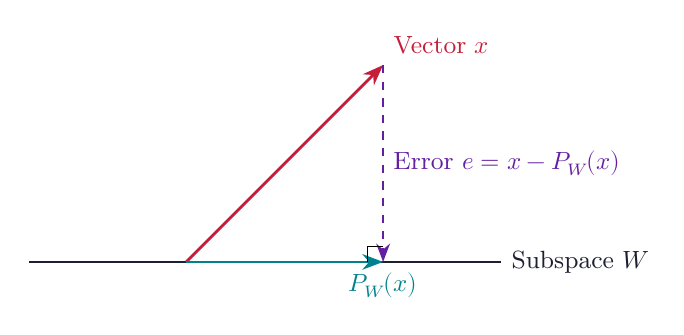
\begin{tikzpicture}[every node/.style={font=\small}]
  % Subspace W (horizontal plane represented by a line)
  \draw[thick, color=mydark] (-2,0) -- (4,0) node[right] {Subspace $W$};
  
  % Vector x (pointing up-right)
  \draw[arrow, color=myred, line width=1pt] (0,0) -- (2.5,2.5) node[above right] {Vector $x$};
  
  % Projection P_W(x)
  \draw[arrow, color=myteal, line width=1pt] (0,0) -- (2.5,0) node[below] {$P_W(x)$};
  
  % Error vector e (vertical dashed arrow)
  \draw[arrow, dashed, color=mypurple, line width=0.8pt] (2.5,2.5) -- (2.5,0) node[midway, right] {Error $e = x - P_W(x)$};
  
  % Orthogonality square indicator
  \draw (2.5,0.2) -- (2.3,0.2) -- (2.3,0);
\end{tikzpicture}
\end{tcolorbox}

\begin{tcolorbox}[examplebox, title={Example: Gram-Schmidt Orthonormalization}]
Apply the Gram-Schmidt process to the following set of vectors in $\mathbb{R}^3$ to obtain an orthonormal basis:
\[
  v_1 = [1, 1, 0]^T, \quad v_2 = [1, 2, 0]^T, \quad v_3 = [0, 1, 2]^T
\]

\textbf{Solution:}
\begin{enumerate}[label=\textbf{\arabic*.}, leftmargin=*, itemsep=4pt]
  \item For $v_1$:
    \[
      u_1 = v_1 = [1, 1, 0]^T \implies \|u_1\| = \sqrt{1^2 + 1^2 + 0^2} = \sqrt{2}
    \]
    \[
      q_1 = \frac{u_1}{\|u_1\|} = \left[\frac{1}{\sqrt{2}}, \frac{1}{\sqrt{2}}, 0\right]^T
    \]
  \item For $v_2$:
    \[
      \langle v_2, q_1 \rangle = (1 \times \frac{1}{\sqrt{2}}) + (2 \times \frac{1}{\sqrt{2}}) + 0 = \frac{3}{\sqrt{2}}
    \]
    \[
      u_2 = v_2 - \langle v_2, q_1 \rangle q_1 = \begin{bmatrix} 1 \\ 2 \\ 0 \end{bmatrix} - \frac{3}{\sqrt{2}}\begin{bmatrix} 1/\sqrt{2} \\ 1/\sqrt{2} \\ 0 \end{bmatrix} = \begin{bmatrix} 1 \\ 2 \\ 0 \end{bmatrix} - \begin{bmatrix} 1.5 \\ 1.5 \\ 0 \end{bmatrix} = \begin{bmatrix} -0.5 \\ 0.5 \\ 0 \end{bmatrix}
    \]
    \[
      \|u_2\| = \sqrt{(-0.5)^2 + 0.5^2 + 0} = \sqrt{0.5} = \frac{1}{\sqrt{2}}
    \]
    \[
      q_2 = \frac{u_2}{\|u_2\|} = \sqrt{2} \begin{bmatrix} -0.5 \\ 0.5 \\ 0 \end{bmatrix} = \left[-\frac{1}{\sqrt{2}}, \frac{1}{\sqrt{2}}, 0\right]^T
    \]
  \item For $v_3$:
    \[
      \langle v_3, q_1 \rangle = \frac{1}{\sqrt{2}}, \quad \langle v_3, q_2 \rangle = \frac{1}{\sqrt{2}}
    \]
    \[
      u_3 = v_3 - \langle v_3, q_1 \rangle q_1 - \langle v_3, q_2 \rangle q_2 = \begin{bmatrix} 0 \\ 1 \\ 2 \end{bmatrix} - \frac{1}{2}\begin{bmatrix} 1 \\ 1 \\ 0 \end{bmatrix} - \frac{1}{2}\begin{bmatrix} -1 \\ 1 \\ 0 \end{bmatrix} = \begin{bmatrix} 0 \\ 0 \\ 2 \end{bmatrix}
    \]
    \[
      \|u_3\| = 2 \implies q_3 = \frac{u_3}{\|u_3\|} = [0, 0, 1]^T
    \]
\end{enumerate}
The orthonormal basis is:
\[
  \left\{ \begin{bmatrix} 1/\sqrt{2} \\ 1/\sqrt{2} \\ 0 \end{bmatrix}, \begin{bmatrix} -1/\sqrt{2} \\ 1/\sqrt{2} \\ 0 \end{bmatrix}, \begin{bmatrix} 0 \\ 0 \\ 1 \end{bmatrix} \right\}
\]
\end{tcolorbox}

% ===============================================================================
% MANDATORY QUICK REVISION PAGE
% ===============================================================================
\newpage
\begin{center}
  {\large\bfseries\color{myred} Quick Revision --- Module III}\\[3pt]
  {\small\color{mydark} LMS Variants \& Signal Space Concepts $|$ PE-EC702A}
\end{center}
\noindent{\color{myred}\rule{\linewidth}{1.2pt}}
\vspace{4pt}

\begin{tcolorbox}[formulabox, title={\textbf{Key Formulas at a Glance}}]
\renewcommand{\arraystretch}{1.3}
\begin{tabularx}{\linewidth}{B{4.5cm} X}
Sign-Error LMS & $\mathbf{w}(n+1) = \mathbf{w}(n) + \mu \operatorname{sgn}(e(n)) \mathbf{x}(n)$ \\[6pt]
Sign-Sign LMS & $\mathbf{w}(n+1) = \mathbf{w}(n) + \mu \operatorname{sgn}(e(n)) \operatorname{sgn}(\mathbf{x}(n))$ \\[6pt]
Normalized LMS Update & $\mathbf{w}(n+1) = \mathbf{w}(n) + \frac{\tilde{\mu}}{\|\mathbf{x}(n)\|^2 + \epsilon} e^*(n) \mathbf{x}(n)$ \\[6pt]
Rank-Nullity Theorem & $\text{rank}(T) + \text{nullity}(T) = \dim(V)$ \\[6pt]
Orthogonal Projection & $P_W(x) = \sum_{i=1}^k \langle x, q_i \rangle q_i$ \quad ($q_i$: orthonormal basis) \\[6pt]
Gram-Schmidt Step & $u_k = v_k - \sum_{j=1}^{k-1} \langle v_k, q_j \rangle q_j, \quad q_k = u_k/\|u_k\|$
\end{tabularx}
\end{tcolorbox}

\begin{tcolorbox}[defbox, title={\textbf{One-Line Definitions}}]
\begin{itemize}[leftmargin=*, itemsep=2.5pt, topsep=0pt]
  \item \textbf{Normalized LMS:} A variant of LMS that divides step-size by input power to maintain stability.
  \item \textbf{Sign-Sign LMS:} A hardware-friendly LMS variant using only signs of data and error.
  \item \textbf{Inner Product Space:} A vector space equipped with a function defining angles and lengths (norms).
  \item \textbf{Gram-Schmidt Process:} An algorithm generating orthonormal bases from a set of linearly independent vectors.
  \item \textbf{Rank of Operator:} The dimension of the range space of a linear transformation.
  \item \textbf{Nullity of Operator:} The dimension of the null space of a linear transformation.
\end{itemize}
\end{tcolorbox}

\begin{tcolorbox}[exambox, title={\textbf{Frequently Asked / Viva Questions}}]
\begin{enumerate}[topsep=0pt, label=\textbf{Q\arabic*.}, itemsep=5pt]
  \item \Q{What is the primary advantage of Sign-LMS algorithms?}
    They reduce hardware multiplier requirements. Sign-Sign LMS replaces the update multiplications with simple addition/subtraction, accelerating hardware processing.
  \item \Q{Why does standard LMS sometimes diverge with speech inputs and how does NLMS solve it?}
    Speech has highly variable power. During high-amplitude segments, the fixed step-size of standard LMS can violate bounds ($2/\text{Tr}(\mathbf{R})$), causing divergence. NLMS scales $\mu$ inversely with instantaneous power, ensuring stability.
  \item \Q{State the Rank-Nullity Theorem.}
    For any linear operator $T: V \to W$ where $V$ is finite-dimensional, $\dim(\mathcal{R}(T)) + \dim(\mathcal{N}(T)) = \dim(V)$, meaning Rank + Nullity = Dimension of domain.
  \item \Q{Explain overlap-save block processing in FDAF.}
    It is a frequency-domain technique that computes block convolutions of input signals with filter weights using DFTs/FFTs, avoiding time-domain convolution overhead.
  \item \Q{What is sub-band adaptive filtering and why is it used?}
    It divides a wideband signal into multiple narrower frequency bands. It speeds up convergence by reducing the eigenvalue spread (whitening) and lowers computational complexity by decimation.
  \item \Q{Define the orthogonal complement of a subspace.}
    The orthogonal complement $W^\perp$ of a subspace $W$ is the set of all vectors in the vector space that are orthogonal to every vector in $W$.
  \item \Q{Write the formula for the orthogonal projection of vector $x$ onto vector $y$.}
    $P_y(x) = \frac{\langle x, y \rangle}{\|y\|^2} y$.
  \item \Q{What represents the inner product of two signals $x(n)$ and $y(n)$ in $L_2$ space?}
    $\langle x, y \rangle = \sum_{n=-\infty}^\infty x(n) y^*(n)$ (for discrete signals) or $\int x(t) y^*(t) dt$ (for continuous signals).
  \item \Q{What is the regularization parameter $\epsilon$ in NLMS?}
    It is a small positive constant added to the denominator to prevent division by zero (or numerical instability) when the input vector norm $\|\mathbf{x}(n)\|$ is zero or very small.
  \item \Q{How does the computational complexity of FDAF scale with filter length $M$?}
    It scales as $O(M \log_2 M)$ compared to $O(M^2)$ for standard time-domain LMS.
\end{enumerate}
\end{tcolorbox}


% -- Module 4 -----------------------------------------------------------------
\modulestart{4}{Vector Space of Random Variables}

\section{Vector Space of Random Variables}
% ===============================================================================

Random variables can be modeled as vectors in a Hilbert space $H$.
\begin{itemize}[leftmargin=*, itemsep=3pt]
  \item \textbf{Inner Product:} For zero-mean random variables $X$ and $Y$, the inner product is defined as their correlation:
  \begin{equation}
    \langle X, Y \rangle = \mathbb{E}[X Y^*]
  \end{equation}
  \item \textbf{Norm:} The norm corresponds to the root-mean-square (RMS) value:
  \begin{equation}
    \|X\| = \sqrt{\langle X, X \rangle} = \sqrt{\mathbb{E}[|X|^2]}
  \end{equation}
  \item \textbf{Orthogonality:} Two random variables are orthogonal if $\langle X, Y \rangle = \mathbb{E}[XY^*] = 0$, meaning they are statistically uncorrelated.
\end{itemize}

% ===============================================================================
\section{Forward and Backward Projections}
% ===============================================================================

Linear prediction involves estimating a signal sample from adjacent samples.

\subsection{Forward Linear Prediction}
Predicts the current sample $x(n)$ based on the past $M$ samples $\{x(n-1), \dots, x(n-M)\}$.
\begin{itemize}[leftmargin=*, itemsep=2pt]
  \item \textbf{Forward Prediction Error ($f_M(n)$):}
  \begin{equation}
    f_M(n) = x(n) - \sum_{k=1}^M a_{M,k}^* x(n-k)
  \end{equation}
  where $a_{M,k}$ are the forward prediction coefficients.
\end{itemize}

\subsection{Backward Linear Prediction}
Predicts the past sample $x(n-M)$ using the current and subsequent $M$ samples $\{x(n), \dots, x(n-M+1)\}$.
\begin{itemize}[leftmargin=*, itemsep=2pt]
  \item \textbf{Backward Prediction Error ($g_M(n)$):}
  \begin{equation}
    g_M(n) = x(n-M) - \sum_{k=1}^M b_{M,k}^* x(n-k+1)
  \end{equation}
  where $b_{M,k}$ are the backward prediction coefficients. For WSS processes, $b_{M,k} = a_{M, M-k+1}^*$.
\end{itemize}

% ===============================================================================
\section{Stochastic Lattice Filters}
% ===============================================================================

Lattice filters represent a modular structure realizing both forward and backward prediction errors order-recursively.

\subsection{Lattice Recursions}
For a stage $m$ (where $m=1, 2, \dots, M$):
\begin{tcolorbox}[defbox, title={Lattice Prediction Error Updates}]
\begin{align}
  f_m(n) &= f_{m-1}(n) - \kappa_m^* g_{m-1}(n-1) \\
  g_m(n) &= g_{m-1}(n-1) - \kappa_m f_{m-1}(n)
\end{align}
Initial conditions for the recursion are: $f_0(n) = g_0(n) = x(n)$.
\end{tcolorbox}
Here, $\kappa_m$ is the \textbf{Reflection Coefficient} (PARCOR coefficient) for stage $m$.

\subsection{Optimal Reflection Coefficients}
To minimize the sum of the forward and backward mean square errors ($\mathbb{E}[|f_m(n)|^2] + \mathbb{E}[|g_m(n)|^2]$), we differentiate with respect to $\kappa_m$, giving:
\begin{equation}
  \kappa_m = \frac{2\mathbb{E}[f_{m-1}(n) g_{m-1}^*(n-1)]}{\mathbb{E}[|f_{m-1}(n)|^2] + \mathbb{E}[|g_{m-1}(n-1)|^2]}
\end{equation}
By Cauchy-Schwarz, $|\kappa_m| \le 1$. This ensures that the all-pole synthesis filter (inverse lattice filter) is guaranteed to be stable if and only if $|\kappa_m| < 1$ for all $m$.

\subsection{Single-Stage Lattice Block Diagram}

\begin{tcolorbox}[tikzbox, title={Lattice Filter Stage $m$ Block Structure}]
\centering
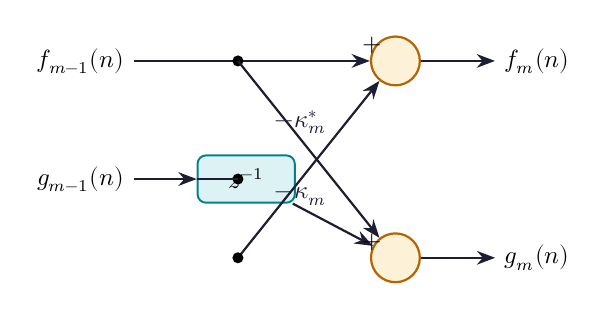
\begin{tikzpicture}[node distance=1.0cm and 1.5cm, every node/.style={font=\small}]
  % Nodes Left (Inputs)
  \node (f_in) at (0, 1.5) {$f_{m-1}(n)$};
  \node (g_in) at (0, 0) {$g_{m-1}(n)$};
  
  % Delay
  \node[block, text width=1.0cm, minimum height=0.6cm, right=0.8cm of g_in] (delay) {$z^{-1}$};
  
  % Junctions
  \node[sumjunc] (sum_f) at (4.0, 1.5) {};
  \node[sumjunc] (sum_g) at (4.0, -1.0) {};
  
  % Connections
  \draw[arrow] (f_in) -- (sum_f);
  \draw[arrow] (g_in) -- (delay);
  
  % Tap points
  \coordinate (tap_f) at (2.0, 1.5);
  \coordinate (tap_g) at (2.0, 0);
  
  \fill (tap_f) circle (2pt);
  \fill (tap_g) circle (2pt);
  
  \draw[arrow] (delay) -- (sum_g);
  
  % Diagonal multiplier paths
  \draw[arrow] (tap_f) -- node[pos=0.7, left, yshift=-0.15cm] {$-\kappa_m$} (sum_g);
  \draw[arrow] (2.0, -1.0) -- node[pos=0.7, left, yshift=0.15cm] {$-\kappa_m^*$} (sum_f);
  \fill (2.0, -1.0) circle (2pt);
  \draw[line] (delay) -- (2.0, 0);
  
  % Outputs
  \node (f_out) at (5.8, 1.5) {$f_m(n)$};
  \node (g_out) at (5.8, -1.0) {$g_m(n)$};
  
  \draw[arrow] (sum_f) -- (f_out);
  \draw[arrow] (sum_g) -- (g_out);
  
  \node at (3.7, 1.7) {$+$};
  \node at (3.7, -0.8) {$+$};
\end{tikzpicture}
\end{tcolorbox}

% ===============================================================================
\section{Relationship with AR Modeling and Levinson-Durbin Recursion}
% ===============================================================================

An Autoregressive (AR) process of order $M$ is generated by filtering white noise through an all-pole filter. The AR parameters and reflection coefficients are equivalent representations of the same process.

\subsection{Levinson-Durbin Recursion}
It solves the Yule-Walker equations $\mathbf{R}\mathbf{a} = \mathbf{r}$ with $O(M^2)$ complexity instead of $O(M^3)$ matrix inversion. The recursion steps for order $m=1, 2, \dots, M$:
\begin{align}
  \Delta_{m-1} &= r(m) - \sum_{i=1}^{m-1} a_{m-1, i} r(m-i) \\
  \kappa_m &= \frac{\Delta_{m-1}}{E_{m-1}} \\
  a_{m, i} &= a_{m-1, i} - \kappa_m a_{m-1, m-i}^* \quad (i=1, \dots, m-1) \\
  a_{m, m} &= \kappa_m \\
  E_m &= E_{m-1}(1 - |\kappa_m|^2)
\end{align}
where $E_0 = r(0)$ is the input variance, and $\kappa_m$ is the reflection coefficient.

% ===============================================================================
\section{Joint Process Estimator and Gradient Adaptive Lattice}
% ===============================================================================

\subsection{Joint Process Estimator (JPE)}
The JPE uses the backward prediction errors $g_m(n)$ of a lattice predictor as the input to a transversal filter to estimate a desired signal $d(n)$. Because the backward errors $\{g_0(n), \dots, g_M(n)\}$ are mutually orthogonal, the estimator weights $h_m$ can be optimized independently:
\begin{equation}
  \hat{d}(n) = \sum_{m=0}^M h_m^* g_m(n), \quad h_m = \frac{\mathbb{E}[d(n)g_m^*(n)]}{\mathbb{E}[|g_m(n)|^2]}
\end{equation}

\subsection{Gradient Adaptive Lattice (GAL)}
GAL is the adaptive implementation of the lattice filter. The reflection coefficients $\kappa_m$ are updated recursively using a stochastic gradient approach:
\begin{align}
  D_m(n) &= \beta D_m(n-1) + (1-\beta) \left[ |f_m(n)|^2 + |g_m(n-1)|^2 \right] \\
  \kappa_{m+1}(n+1) &= \kappa_{m+1}(n) + \frac{\mu}{D_m(n)} \left[ f_m(n) g_m^*(n-1) \right]
\end{align}
where $\beta$ is a smoothing factor and $D_m(n)$ estimates the power at stage $m$.

\begin{tcolorbox}[examplebox, title={Example: Levinson-Durbin Recursion}]
Given autocorrelation values $r(0) = 1.0, r(1) = 0.5, r(2) = 0.125$. Run the Levinson-Durbin recursion to find the reflection coefficients $\kappa_1, \kappa_2$ and the predictor coefficients of a second-order predictor.

\textbf{Solution:}
Initialize: $E_0 = r(0) = 1.0$.
\textbf{Iteration 1 ($m=1$):}
\[
  \Delta_0 = r(1) = 0.5
\]
\[
  \kappa_1 = \frac{\Delta_0}{E_0} = \frac{0.5}{1.0} = 0.5
\]
Predictor coefficient:
\[
  a_{1,1} = \kappa_1 = 0.5
\]
Update error energy:
\[
  E_1 = E_0(1 - \kappa_1^2) = 1.0(1 - 0.25) = 0.75
\]
\textbf{Iteration 2 ($m=2$):}
\[
  \Delta_1 = r(2) - a_{1,1}r(1) = 0.125 - (0.5 \times 0.5) = 0.125 - 0.25 = -0.125
\]
\[
  \kappa_2 = \frac{\Delta_1}{E_1} = \frac{-0.125}{0.75} = -\frac{1}{6} \approx -0.1667
\]
Predictor coefficients:
\[
  a_{2,2} = \kappa_2 = -0.1667
\]
\[
  a_{2,1} = a_{1,1} - \kappa_2 a_{1,1} = 0.5 - \left(-\frac{1}{6} \times 0.5\right) = 0.5 + 0.0833 = 0.5833
\]
Update error energy:
\[
  E_2 = E_1(1 - \kappa_2^2) = 0.75 \left(1 - \frac{1}{36}\right) = 0.75 \times \frac{35}{36} = 0.7292
\]
The reflection coefficients are $\kappa_1 = 0.5, \kappa_2 = -0.1667$, and predictor coefficients are $a_{2,1} = 0.5833, a_{2,2} = -0.1667$.
\end{tcolorbox}

% ===============================================================================
% MANDATORY QUICK REVISION PAGE
% ===============================================================================
\newpage
\begin{center}
  {\large\bfseries\color{myred} Quick Revision --- Module IV}\\[3pt]
  {\small\color{mydark} Lattice Filters \& Linear Prediction $|$ PE-EC702A}
\end{center}
\noindent{\color{myred}\rule{\linewidth}{1.2pt}}
\vspace{4pt}

\begin{tcolorbox}[formulabox, title={\textbf{Key Formulas at a Glance}}]
\renewcommand{\arraystretch}{1.3}
\begin{tabularx}{\linewidth}{B{4.5cm} X}
Forward Error & $f_m(n) = f_{m-1}(n) - \kappa_m^* g_{m-1}(n-1)$ \\[6pt]
Backward Error & $g_m(n) = g_{m-1}(n-1) - \kappa_m f_{m-1}(n)$ \\[6pt]
Reflection Coeff. ($\kappa_m$) & $\kappa_m = \frac{2\mathbb{E}[f_{m-1}(n) g_{m-1}^*(n-1)]}{\mathbb{E}[|f_{m-1}(n)|^2] + \mathbb{E}[|g_{m-1}(n-1)|^2]}$ \\[6pt]
Levinson-Durbin $\kappa_m$ & $\kappa_m = \Delta_{m-1}/E_{m-1}$ \\[6pt]
Predictor Coefficient Update & $a_{m, i} = a_{m-1, i} - \kappa_m a_{m-1, m-i}^*$ \quad ($a_{m,m} = \kappa_m$) \\[6pt]
Error Energy Update & $E_m = E_{m-1}(1 - |\kappa_m|^2)$
\end{tabularx}
\end{tcolorbox}

\begin{tcolorbox}[defbox, title={\textbf{One-Line Definitions}}]
\begin{itemize}[leftmargin=*, itemsep=2.5pt, topsep=0pt]
  \item \textbf{Forward Prediction Error:} The difference between the current signal sample and its linear estimate based on past samples.
  \item \textbf{Backward Prediction Error:} The difference between a past signal sample and its estimate based on subsequent samples.
  \item \textbf{Reflection Coefficient:} The correlation metric $\kappa_m$ bounded in $[-1, 1]$ parameterizing a lattice stage.
  \item \textbf{Levinson-Durbin Recursion:} An efficient $O(M^2)$ recursive algorithm to solve the Yule-Walker equations.
  \item \textbf{Joint Process Estimator:} A structure utilizing orthogonal backward errors to estimate an external desired signal.
  \item \textbf{GAL Filter:} A gradient-based adaptive lattice filter that adjusts reflection coefficients stage-by-stage.
\end{itemize}
\end{tcolorbox}

\begin{tcolorbox}[exambox, title={\textbf{Frequently Asked / Viva Questions}}]
\begin{enumerate}[topsep=0pt, label=\textbf{Q\arabic*.}, itemsep=5pt]
  \item \Q{What are the initial conditions for the lattice filter recursions?}
    $f_0(n) = g_0(n) = x(n)$, representing the raw input sample.
  \item \Q{Explain why lattice filters are preferred in hardware over transversal (FIR) filters.}
    Lattice filters are modular. Increasing the filter order simply requires adding more identical stages at the end, without recalculating prior stages' coefficients.
  \item \Q{What condition must reflection coefficients satisfy to ensure system stability?}
    $|\kappa_m| < 1$ for all stages $m$. If any $|\kappa_m| \ge 1$, the corresponding synthesis filter becomes unstable.
  \item \Q{Why are backward prediction errors $g_m(n)$ orthogonal to each other?}
    Because $g_m(n)$ represents the component of $x(n-m)$ that is orthogonal to the subspace spanned by $\{x(n), \dots, x(n-m+1)\}$. Thus, $\mathbb{E}[g_i(n)g_j^*(n)] = 0$ for $i \ne j$.
  \item \Q{How does the computational complexity of Levinson-Durbin compare to direct matrix inversion?}
    Levinson-Durbin requires $O(M^2)$ operations, whereas direct inversion of the correlation matrix via Gaussian elimination requires $O(M^3)$ operations.
  \item \Q{What is the relationship between predictor coefficients and reflection coefficients?}
    Predictor coefficients $a_{M,k}$ are calculated from reflection coefficients $\kappa_m$ using the step-up recursion relation: $a_{m,i} = a_{m-1,i} - \kappa_m a_{m-1,m-i}^*$.
  \item \Q{What is a Joint Process Estimator (JPE)?}
    It is an adaptive structure that first orthogonalizes the input signal using a lattice filter, and then estimates a desired response by forming a weighted linear combination of the orthogonal backward prediction errors.
  \item \Q{Define the PARCOR coefficient.}
    It stands for PARTial CORrelation coefficient, which is mathematically identical to the reflection coefficient $\kappa_m$ in a lattice filter.
  \item \Q{Why does the error energy $E_m$ decrease with increase in predictor order $m$?}
    Because $E_m = E_{m-1}(1 - |\kappa_m|^2)$, and since $|\kappa_m| < 1$, the factor $(1 - |\kappa_m|^2) \le 1$, meaning adding more taps can only reduce (or keep equal) the prediction error power.
  \item \Q{What is the role of the power estimator $D_m(n)$ in the GAL algorithm?}
    It normalizes the step-size for each stage individually (similar to NLMS), ensuring that convergence speed is uniform across all stages regardless of local signal power.
\end{enumerate}
\end{tcolorbox}

\begin{tcolorbox}[tikzbox, title={Comparison of Transversal vs. Lattice Predictor Structures}]
\renewcommand{\arraystretch}{1.45}
\par\noindent
\begin{tabularx}{\linewidth}{|B{3.2cm}|Y|Y|}
\hline
\rowcolor{hdrgray}
\textbf{Property} & \textbf{Transversal (Tapped Delay Line)} & \textbf{Lattice Structure} \\
\hline
\textbf{Modularity} & Low (adding a tap changes all weights) & High (adding a tap is just adding a stage) \\
\hline
\textbf{Stability Check} & Complex (requires finding roots of polynomial) & Simple (checks if $|\kappa_m| < 1$ for all stages) \\
\hline
\textbf{Numerical Sensitivity} & High (sensitive to coefficient quantization) & Low (robust to finite word-length effects) \\
\hline
\textbf{Complexity} & $O(M)$ multiplications per update & $O(M)$ multiplications per update (slightly higher constant) \\
\hline
\end{tabularx}
\end{tcolorbox}


% -- Module 5 -----------------------------------------------------------------
\modulestart{5}{Introduction to Recursive Least Squares (RLS)}

\section{Introduction to Recursive Least Squares (RLS)}
% ===============================================================================

The Recursive Least Squares (RLS) algorithm minimizes a deterministic, exponentially weighted sum of squared errors, rather than statistical ensemble averages. 

\subsection{RLS Cost Function}
The cost function to minimize at time $n$ is:
\begin{equation}
  \mathcal{E}(n) = \sum_{i=1}^n \lambda^{n-i} |e(i, n)|^2
\end{equation}
where $\lambda \in (0, 1]$ is the \textbf{exponential forgetting factor} (typically $0.95 \le \lambda \le 1.0$), and the error signal is $e(i, n) = d(i) - \mathbf{w}^H(n) \mathbf{x}(i)$ for $i=1, 2, \dots, n$, using the weight vector at current time $n$.

\subsection{Least-Squares Normal Equations}
Setting the gradient of $\mathcal{E}(n)$ with respect to $\mathbf{w}^*$ to zero yields the deterministic normal equations:
\begin{equation}
  \mathbf{\Phi}(n) \mathbf{w}(n) = \mathbf{z}(n) \implies \mathbf{w}(n) = \mathbf{\Phi}^{-1}(n) \mathbf{z}(n)
\end{equation}
where the deterministic correlation matrix $\mathbf{\Phi}(n)$ and cross-correlation vector $\mathbf{z}(n)$ are:
\begin{align}
  \mathbf{\Phi}(n) &= \sum_{i=1}^n \lambda^{n-i} \mathbf{x}(i) \mathbf{x}^H(i) = \lambda \mathbf{\Phi}(n-1) + \mathbf{x}(n) \mathbf{x}^H(n) \\
  \mathbf{z}(n) &= \sum_{i=1}^n \lambda^{n-i} \mathbf{x}(i) d^*(i) = \lambda \mathbf{z}(n-1) + \mathbf{x}(n) d^*(n)
\end{align}

% ===============================================================================
\section{Vector Space Formulation of RLS and Matrix Inversion Lemma}
% ===============================================================================

\subsection{Matrix Inversion Lemma (Woodbury Identity)}
To update $\mathbf{\Phi}^{-1}(n)$ without direct inversion, we use the Matrix Inversion Lemma:
\begin{equation}
  (\mathbf{A} + \mathbf{B}\mathbf{C}\mathbf{D})^{-1} = \mathbf{A}^{-1} - \mathbf{A}^{-1}\mathbf{B}(\mathbf{C}^{-1} + \mathbf{D}\mathbf{A}^{-1}\mathbf{B})^{-1}\mathbf{D}\mathbf{A}^{-1}
\end{equation}
By defining $\mathbf{P}(n) = \mathbf{\Phi}^{-1}(n)$ and substituting $\mathbf{A} = \lambda \mathbf{\Phi}(n-1)$, $\mathbf{B} = \mathbf{x}(n)$, $\mathbf{C} = 1$, and $\mathbf{D} = \mathbf{x}^H(n)$, we obtain:
\begin{equation}
  \mathbf{P}(n) = \lambda^{-1} \mathbf{P}(n-1) - \frac{\lambda^{-2}\mathbf{P}(n-1)\mathbf{x}(n)\mathbf{x}^H(n)\mathbf{P}(n-1)}{1 + \lambda^{-1}\mathbf{x}^H(n)\mathbf{P}(n-1)\mathbf{x}(n)}
\end{equation}

\subsection{The Gain Vector}
Defining the gain vector $\mathbf{k}(n)$ as:
\begin{equation}
  \mathbf{k}(n) = \frac{\mathbf{P}(n-1)\mathbf{x}(n)}{\lambda + \mathbf{x}^H(n)\mathbf{P}(n-1)\mathbf{x}(n)} = \mathbf{P}(n)\mathbf{x}(n)
\end{equation}
Allows writing the inverse correlation update compactly as:
\begin{equation}
  \mathbf{P}(n) = \lambda^{-1} \left[ \mathbf{P}(n-1) - \mathbf{k}(n) \mathbf{x}^H(n) \mathbf{P}(n-1) \right]
\end{equation}

% ===============================================================================
\section{RLS Transversal Adaptive Filter Algorithm}
% ===============================================================================

The complete step-by-step transversal RLS algorithm is structured as follows:

\begin{tcolorbox}[defbox, title={RLS Algorithm Steps}]
\textbf{Initialization (at $n=0$):}
\begin{align}
  \mathbf{w}(0) &= \mathbf{0} \\
  \mathbf{P}(0) &= \delta^{-1} \mathbf{I} \quad (\delta \text{ is a small positive constant})
\end{align}
\textbf{Recursion (for each time index $n=1, 2, \dots$):}
\begin{enumerate}[label=\textbf{\arabic*.}, leftmargin=*, itemsep=3pt]
  \item Compute the gain vector:
  \[
    \mathbf{k}(n) = \frac{\mathbf{P}(n-1)\mathbf{x}(n)}{\lambda + \mathbf{x}^H(n)\mathbf{P}(n-1)\mathbf{x}(n)}
  \]
  \item Calculate the a priori estimation error:
  \[
    \xi(n) = d(n) - \mathbf{w}^H(n-1)\mathbf{x}(n)
  \]
  \item Update the filter weights:
  \[
    \mathbf{w}(n) = \mathbf{w}(n-1) + \mathbf{k}(n)\xi^*(n)
  \]
  \item Update the inverse correlation matrix:
  \[
    \mathbf{P}(n) = \lambda^{-1} \left[ \mathbf{P}(n-1) - \mathbf{k}(n)\mathbf{x}^H(n)\mathbf{P}(n-1) \right]
  \]
\end{enumerate}
\end{tcolorbox}

\subsection{RLS Lattice Filters}
RLS lattice filters (Least-Squares Lattice, LSL) combine the fast convergence of least-squares algorithms with the modular, low-computational complexity $O(M)$ of lattice structures, solving numerical sensitivity issues of standard RLS.

% ===============================================================================
\section{Advanced Topics}
% ===============================================================================

\subsection{Affine Projection Algorithm (APA)}
APA generalizes NLMS. Instead of adjusting the weight vector based on the current input vector $\mathbf{x}(n)$, APA projects the weights onto a subspace spanned by $P$ past input vectors (where $P$ is the projection order).
\begin{itemize}[leftmargin=*, itemsep=2pt]
  \item \textbf{Significance:} For $P=1$, APA reduces to NLMS. For $P=M$ (filter length), it approaches RLS performance. It offers a flexible trade-off between computational complexity and convergence speed for highly correlated inputs.
\end{itemize}

\subsection{Subspace-Based Adaptive Filters}
These algorithms decompose the signal space into orthogonal signal and noise subspaces using eigendecomposition or singular value decomposition (SVD). By projecting updates exclusively onto the signal subspace, it filters out noise components, enhancing performance in high-resolution estimation tasks.

\subsection{Partial Update Algorithms}
To save power and processor cycles in resource-constrained environments (e.g., mobile devices), these algorithms update only a subset of the $M$ filter coefficients at each iteration, selecting either a fixed subset (Periodic LMS) or a dynamic subset based on magnitude (Max-NLMS).

\subsection{QR Decomposition (QRD-RLS) and Systolic Arrays}
Standard RLS is numerically unstable under finite word-length effects because the matrix $\mathbf{P}(n)$ can lose its positive-definiteness due to round-off errors.
\begin{itemize}[leftmargin=*, itemsep=3pt]
  \item \textbf{QRD-RLS:} Solves the least-squares problem by applying unitary transformations (Givens rotations) directly to the data matrix $\mathbf{X}(n)$, decomposing it into an orthogonal matrix $\mathbf{Q}(n)$ and an upper triangular matrix $\mathbf{R}(n)$. Since unitary transformations preserve norms, QRD-RLS is numerically stable.
  \item \textbf{Systolic Arrays:} A systolic array is a parallel network of processors (Boundary Cells and Internal Cells) that pipelined Givens rotations for real-time QRD-RLS VLSI hardware execution.
\end{itemize}

\begin{tcolorbox}[tikzbox, title={Systolic Array Structure for QRD-RLS}]
\centering
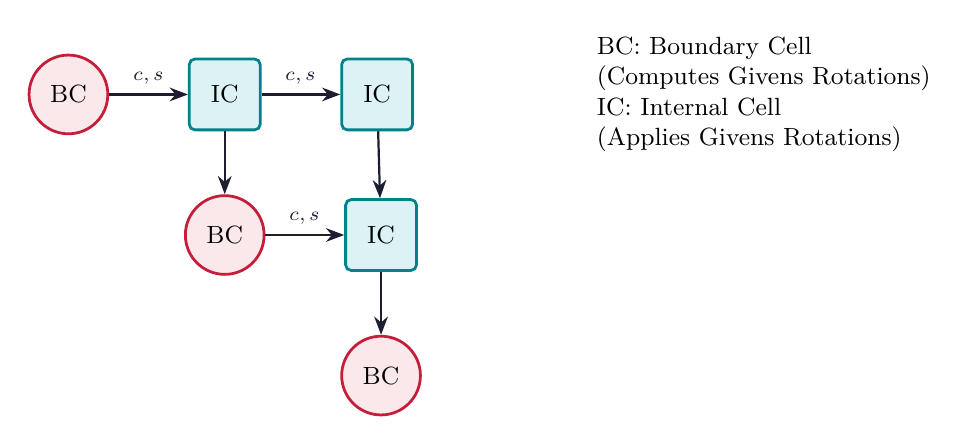
\begin{tikzpicture}[node distance=1.2cm and 1.2cm, every node/.style={font=\small}]
  % Boundary cell (circle)
  \node[circle, draw=myred, fill=hdrred, minimum size=1.0cm, line width=1.0pt] (bc1) at (0,0) {BC};
  
  % Internal cells (squares)
  \node[rectangle, draw=myteal, fill=hdrteal, minimum size=0.9cm, right=1.0cm of bc1, rounded corners=2pt, line width=1.0pt] (ic1) {IC};
  \node[rectangle, draw=myteal, fill=hdrteal, minimum size=0.9cm, right=1.0cm of ic1, rounded corners=2pt, line width=1.0pt] (ic2) {IC};
  
  \node[circle, draw=myred, fill=hdrred, minimum size=1.0cm, below=0.8cm of ic1, line width=1.0pt] (bc2) {BC};
  \node[rectangle, draw=myteal, fill=hdrteal, minimum size=0.9cm, right=1.0cm of bc2, rounded corners=2pt, line width=1.0pt] (ic3) {IC};
  
  \node[circle, draw=myred, fill=hdrred, minimum size=1.0cm, below=0.8cm of ic3, line width=1.0pt] (bc3) {BC};
  
  % Connections
  \draw[arrow] (bc1) -- node[above, font=\scriptsize] {$c, s$} (ic1);
  \draw[arrow] (ic1) -- node[above, font=\scriptsize] {$c, s$} (ic2);
  
  \draw[arrow] (bc2) -- node[above, font=\scriptsize] {$c, s$} (ic3);
  
  \draw[arrow] (ic1) -- (bc2);
  \draw[arrow] (ic2) -- (ic3);
  \draw[arrow] (ic3) -- (bc3);
  
  % Legend labels
  \node[right=2.2cm of ic2, align=left] {BC: Boundary Cell \\ (Computes Givens Rotations) \\ IC: Internal Cell \\ (Applies Givens Rotations)};
\end{tikzpicture}
\end{tcolorbox}

\begin{tcolorbox}[examplebox, title={Example: RLS Iteration Computation}]
Given $\lambda = 1.0$, the current estimate $\mathbf{w}(n-1) = [0.5, -0.2]^T$, and the inverse correlation matrix:
\[
  \mathbf{P}(n-1) = \begin{bmatrix} 2.0 & 0.5 \\ 0.5 & 1.0 \end{bmatrix}
\]
The new input sample vector is $\mathbf{x}(n) = [1.0, 2.0]^T$, and the desired signal is $d(n) = 0.8$. Execute one step of the RLS recursion to find the updated weight vector $\mathbf{w}(n)$.

\textbf{Solution:}
\begin{enumerate}[label=\textbf{\arabic*.}, leftmargin=*, itemsep=4pt]
  \item Compute the numerator of the gain vector:
    \[
      \mathbf{P}(n-1)\mathbf{x}(n) = \begin{bmatrix} 2.0 & 0.5 \\ 0.5 & 1.0 \end{bmatrix} \begin{bmatrix} 1.0 \\ 2.0 \end{bmatrix} = \begin{bmatrix} (2 \times 1) + (0.5 \times 2) \\ (0.5 \times 1) + (1 \times 2) \end{bmatrix} = \begin{bmatrix} 3.0 \\ 2.5 \end{bmatrix}
    \]
  \item Compute the denominator of the gain vector:
    \[
      \lambda + \mathbf{x}^T(n)\mathbf{P}(n-1)\mathbf{x}(n) = 1.0 + \begin{bmatrix} 1.0 & 2.0 \end{bmatrix} \begin{bmatrix} 3.0 \\ 2.5 \end{bmatrix} = 1.0 + (3.0 + 5.0) = 9.0
    \]
  \item Compute the gain vector $\mathbf{k}(n)$:
    \[
      \mathbf{k}(n) = \frac{1}{9.0} \begin{bmatrix} 3.0 \\ 2.5 \end{bmatrix} = \begin{bmatrix} 1/3 \\ 5/18 \end{bmatrix} \approx \begin{bmatrix} 0.3333 \\ 0.2778 \end{bmatrix}
    \]
  \item Compute the a priori estimation error $\xi(n)$:
    \[
      \xi(n) = d(n) - \mathbf{w}^T(n-1)\mathbf{x}(n) = 0.8 - \begin{bmatrix} 0.5 & -0.2 \end{bmatrix} \begin{bmatrix} 1.0 \\ 2.0 \end{bmatrix} = 0.8 - (0.5 - 0.4) = 0.7
    \]
  \item Update the weight vector $\mathbf{w}(n)$:
    \[
      \mathbf{w}(n) = \mathbf{w}(n-1) + \mathbf{k}(n)\xi(n) = \begin{bmatrix} 0.5 \\ -0.2 \end{bmatrix} + 0.7 \begin{bmatrix} 1/3 \\ 5/18 \end{bmatrix} = \begin{bmatrix} 0.5 + 0.2333 \\ -0.2 + 0.1944 \end{bmatrix} = \begin{bmatrix} 0.7333 \\ -0.0056 \end{bmatrix}
    \]
\end{enumerate}
\end{tcolorbox}

% ===============================================================================
% MANDATORY QUICK REVISION PAGE
% ===============================================================================
\newpage
\begin{center}
  {\large\bfseries\color{myred} Quick Revision --- Module V}\\[3pt]
  {\small\color{mydark} Recursive Least Squares (RLS) \& Advanced Topics $|$ PE-EC702A}
\end{center}
\noindent{\color{myred}\rule{\linewidth}{1.2pt}}
\vspace{4pt}

\begin{tcolorbox}[formulabox, title={\textbf{Key Formulas at a Glance}}]
\renewcommand{\arraystretch}{1.3}
\begin{tabularx}{\linewidth}{B{4.5cm} X}
RLS Cost Function & $\mathcal{E}(n) = \sum_{i=1}^n \lambda^{n-i} |e(i, n)|^2$ \\[6pt]
Correlation Matrix Update & $\mathbf{\Phi}(n) = \lambda \mathbf{\Phi}(n-1) + \mathbf{x}(n)\mathbf{x}^H(n)$ \\[6pt]
Matrix Inversion Lemma & $(\mathbf{A} + \mathbf{B}\mathbf{C}\mathbf{D})^{-1} = \mathbf{A}^{-1} - \mathbf{A}^{-1}\mathbf{B}(\mathbf{C}^{-1} + \mathbf{D}\mathbf{A}^{-1}\mathbf{B})^{-1}\mathbf{D}\mathbf{A}^{-1}$ \\[6pt]
Gain Vector $\mathbf{k}(n)$ & $\mathbf{k}(n) = \frac{\mathbf{P}(n-1)\mathbf{x}(n)}{\lambda + \mathbf{x}^H(n)\mathbf{P}(n-1)\mathbf{x}(n)}$ \\[6pt]
Weight Update & $\mathbf{w}(n) = \mathbf{w}(n-1) + \mathbf{k}(n)\xi^*(n)$ \quad ($\xi(n) = d(n) - \mathbf{w}^H(n-1)\mathbf{x}(n)$) \\[6pt]
Inverse Matrix Update & $\mathbf{P}(n) = \lambda^{-1} \left[ \mathbf{P}(n-1) - \mathbf{k}(n)\mathbf{x}^H(n)\mathbf{P}(n-1) \right]$
\end{tabularx}
\end{tcolorbox}

\begin{tcolorbox}[defbox, title={\textbf{One-Line Definitions}}]
\begin{itemize}[leftmargin=*, itemsep=2.5pt, topsep=0pt]
  \item \textbf{RLS Algorithm:} An adaptive filter algorithm that recursively finds coefficients to minimize deterministic sum of squared errors.
  \item \textbf{Forgetting Factor:} A scalar parameter $\lambda \le 1.0$ weighting recent data samples more heavily than older ones.
  \item \textbf{Gain Vector:} The vector $\mathbf{k}(n)$ that scales the error term in the RLS weight update equation.
  \item \textbf{Matrix Inversion Lemma:} A mathematical formula allowing recursive computation of matrix inverses without direct inversion.
  \item \textbf{Systolic Array:} A network of processing elements configured to execute parallel QRD matrix operations in hardware.
  \item \textbf{Boundary Cell:} A processor in a QRD systolic array calculating Givens rotation parameters (cosines and sines).
\end{itemize}
\end{tcolorbox}

\begin{tcolorbox}[exambox, title={\textbf{Frequently Asked / Viva Questions}}]
\begin{enumerate}[topsep=0pt, label=\textbf{Q\arabic*.}, itemsep=5pt]
  \item \Q{Compare RLS and LMS in terms of convergence speed and computational complexity.}
    RLS converges much faster than LMS (typically within $2M$ iterations, independent of eigenvalue spread) but requires higher computational complexity ($O(M^2)$ multiplications per sample compared to $O(M)$ for LMS).
  \item \Q{Explain the role of the forgetting factor $\lambda$ in the RLS cost function.}
    $\lambda$ determines the memory of the filter. If $\lambda = 1.0$, the filter has infinite memory (all data weighted equally). If $\lambda < 1.0$ (typically $0.98$), older data is exponentially attenuated, allowing the filter to track non-stationary changes.
  \item \Q{Write down the Woodbury identity (Matrix Inversion Lemma) and explain its use in RLS.}
    $(\mathbf{A} + \mathbf{U}\mathbf{C}\mathbf{V})^{-1} = \mathbf{A}^{-1} - \mathbf{A}^{-1}\mathbf{U}(\mathbf{C}^{-1} + \mathbf{V}\mathbf{A}^{-1}\mathbf{U})^{-1}\mathbf{V}\mathbf{A}^{-1}$. It is used to recursively update the inverse correlation matrix $\mathbf{P}(n) = \mathbf{\Phi}^{-1}(n)$ without performing an $O(M^3)$ matrix inversion step.
  \item \Q{What are the typical initialization values for the RLS algorithm?}
    $\mathbf{w}(0) = \mathbf{0}$ and $\mathbf{P}(0) = \delta^{-1}\mathbf{I}$, where $\delta$ is a small positive regularization parameter (e.g., $0.01$).
  \item \Q{What is the difference between a priori error $\xi(n)$ and a posteriori error $e(n)$ in RLS?}
    The a priori error $\xi(n) = d(n) - \mathbf{w}^H(n-1)\mathbf{x}(n)$ is calculated using the old weight vector, while the a posteriori error $e(n) = d(n) - \mathbf{w}^H(n)\mathbf{x}(n)$ is calculated using the updated weight vector.
  \item \Q{What is the purpose of using QR Decomposition (QRD) in RLS filters?}
    Standard RLS suffers from numerical instability under finite precision arithmetic, causing $\mathbf{P}(n)$ to lose positive-definiteness. QRD solves this by applying unitary rotations to the data matrix, ensuring numerical stability.
  \item \Q{What is the Affine Projection Algorithm (APA)?}
    APA is an intermediate algorithm between NLMS and RLS that updates weights based on the current and $P-1$ past input vectors, speeding up convergence for correlated signals with moderate complexity.
  \item \Q{What are partial update algorithms and where are they useful?}
    They are algorithms that update only a fraction of the filter weights at each time index to reduce power consumption and processing requirements, useful in acoustic echo cancellation in mobile phones.
  \item \Q{What are the functions of boundary cells and internal cells in a systolic array?}
    Boundary cells compute the Givens rotation parameters (cosine $c$ and sine $s$) to zero out elements of the incoming data matrix, while internal cells apply these rotations to the rest of the matrix rows.
  \item \Q{Why does RLS converge independently of the eigenvalue spread of the input signal?}
    Because RLS pre-whitens the input signal by multiplying the error vector with the inverse correlation matrix $\mathbf{P}(n)$, which de-correlates the input modes.
\end{enumerate}
\end{tcolorbox}

\begin{tcolorbox}[tikzbox, title={Comparison of LMS vs. RLS Algorithms}]
\renewcommand{\arraystretch}{1.45}
\par\noindent
\begin{tabularx}{\linewidth}{|B{3.2cm}|Y|Y|}
\hline
\rowcolor{hdrgray}
\textbf{Parameter} & \textbf{LMS Algorithm} & \textbf{RLS Algorithm} \\
\hline
\textbf{Convergence Rate} & Slow (dependent on input eigenvalue spread) & Fast (typically within $2M$ iterations, independent of spread) \\
\hline
\textbf{Complexity} & $O(M)$ multiplications per sample & $O(M^2)$ multiplications per sample \\
\hline
\textbf{Stability} & Stable if $0 < \mu < 2/\text{Tr}(\mathbf{R})$ & Can suffer from numerical instability in finite precision \\
\hline
\textbf{Parameters} & Step-size $\mu$ & Forgetting factor $\lambda$, regularization $\delta$ \\
\hline
\end{tabularx}
\end{tcolorbox}


\end{document}
